\chapter{Password Guessing Algorithms}
\label{chp5::password-guessing-algorithms}

In the previous chapter, we performed an analysis of password composition, which reinforced \textit{why} passwords are guessable. We also demonstrated how secure, yet memorable, passwords can be created. This chapter will focus on \textit{how} passwords are guessed by examining the techniques and algorithms used. We aim to determine whether the guessing techniques described in the literature are practical and whether they add any value to password security. We provide the first systematic overview of techniques and guessing algorithms used in both industry~and~academia.

\section{Introduction}
\label{sec::chp5::introduction}

Although significant research has focused on the composition and creation of passwords, the techniques used to guess or crack these passwords are equally important for understanding password security. However, we rarely see academic password guessing algorithms deployed and used in practice\footnote{We have only encountered \markovngram and \pcfg used in the wild.}, suggesting problems with existing approaches. So, we hypothesise that academic password guessing methods might be misaligned with practical requirements and therefore require a new form of benchmark. We investigate this in Section~\ref{sec::chp5::process}, where we combine the quality of the candidate passwords generated with the generation speed.

\noteBox{Preimage Attack}{
Password guessing can be formalized as a preimage search problem: given a hash value $y$, find an input $x$ such that $h(x) = y$, where $h$ is a cryptographic hash function and $x$ is the target password.
}
\paragraph{Problems\;with\;Existing\;Approaches.}\;A trivial solution for password guessing is an exhaustive search (brute force), but this is computationally infeasible for even moderate password lengths. More sophisticated approaches leverage patterns in human-chosen passwords to reduce the search space. However, existing techniques suffer from several drawbacks:

\begin{itemize}
\item Academic password guessing algorithms often prioritise candidate quality over generation speed, making them impractical for real-world applications where speed is critical.
\item Many proposed techniques lack reproducibility and proper experimental controls, making it difficult to fairly compare different approaches.
\item There is a significant disconnect between academic research and industry practice, with theoretical advances rarely translating to practical improvements.
\end{itemize}

Our aim is to systematically analyse password guessing algorithms in order to: 1) Provide a comprehensive overview and system for existing techniques and algorithms. 2) Establish a model to benchmark methods and algorithms that takes into account the quality and speed of candidate generation.


In this chapter, we provide a systematisation of knowledge (SoK) of password guessing algorithms that bridges the gap between academic research and practical application. Our work provides:
\begin{itemize}
\item A unified framework for understanding and categorising password guessing algorithms.
\item A framework that combines generation quality with generation speed to better measure the effective performance of password guessing algorithms.
\item A detailed overview of \textit{Mask Attack} and their performance using the \pwdninja data set created in Chapter~\ref{chp4::password-composition}.
\end{itemize}
%%%\section{Background}
\label{chp5::sec::background}

The concept of computer passwords was first introduced in the 1960s with the Compatible Time-Sharing System (CTSS) at MIT. However, it wasn't until 1979 that dictionary attacks were first discussed by Robert Morris and Ken Thompson in their paper "Password security: a case history" [1]. They also proposed the first example of password rules to enhance security.

In the early days of password cracking, tools like Crack, released by Alec Muffet in 1992, performed dictionary attacks against Unix passwords using lists of commonly used passwords, demonstrating the vulnerability of weak password practices. In 1989-1992, Klein [2][3] conducted a study where he ran dictionary attacks against a set of ~15,000 encrypted passwords contributed by volunteers. Using a dictionary of approximately 62,000 words, Klein successfully cracked around 39% of the passwords.

As technology advanced, more sophisticated tools emerged. In 2003, Philippe Oechslin released RainbowCrack, which implemented rainbow tables to crack passwords efficiently. Rainbow tables are precomputed tables that store the hashes of plaintext passwords, allowing for faster password cracking. In 2009, oclHashcat was released, leveraging the power of GPUs to significantly increase the speed of password cracking.

With the increasing adoption of the internet and web applications from 2010 onwards, data breaches and cyber crimes became more prevalent, resulting in a larger number of passwords being leaked into the wild. This abundance of real-world password data has facilitated the development of more advanced password guessing techniques.

Password guessing techniques have evolved alongside progress in deep learning and other machine learning methods. However, the utilization of powerful hardware, such as GPUs, has proven to be more effective in practice, leading to a widening gap between industry and academia in terms of password cracking capabilities.

To combat the growing threats to password security, various countermeasures have been developed. Salting, which involves appending a unique random value to each password before hashing, helps prevent attacks using precomputed tables like rainbow tables. Key derivation functions, such as PBKDF2, bcrypt, scrypt, and Argon2, have been designed to slow down the password cracking process by increasing the computational cost of hash calculations.

Several software tools have been developed to assist in password cracking and security testing. Hashcat, originally released as a CPU-based tool for cracking WPA/WPA2 protocols and later made open-source in 2015, has become one of the most popular password cracking tools. John the Ripper (JtR), designed by Alexander Peslyak to detect weak Unix passwords, is another widely used tool. Other notable tools include Aircrack-ng, primarily used for Wi-Fi protocols; Cain \& Abel; Ophcrack; THC Hydra; L0phtCrack; and Medusa.

Mathematically, the password cracking process can be represented as follows:

Let $P$ be the set of all possible plaintext passwords, and $H$ be the set of corresponding password hashes. The goal of password cracking is to find a function $f: H \rightarrow P$ that maps a given password hash $h \in H$ to its original plaintext password $p \in P$, such that $hash(p) = h$.

The efficiency of password cracking techniques can be measured by the number of guesses required to find the correct password, denoted as $G$. The objective is to minimize $G$ by using various strategies, such as dictionary attacks, rule-based attacks, and probabilistic models, to prioritize the most likely password candidates.

In summary, the history of password guessing has been shaped by the interplay between advancements in technology, the increasing availability of password data, and the development of countermeasures. As the field continues to evolve, it is crucial to stay informed about the latest techniques and best practices in password security to protect against emerging threats.

%%%\section{Game of Passwords}

In this section we outline a password gaming. The minimum number of questions to ask in order to guess their password with a high $\mathbb{P}$ in $x$ guesses.

Like the wordle game, what information about the target password would reveal useful info and therefore reduce the search space?

\begin{itemize}
    \item Length
    \item Structure
    \item Character placements
    \item Language
    \item Personal information (PII), e.g. date of birth.
\end{itemize}

Our assumptions are: 1) the passwords are user generated, 2) we are not allowed to ask what the password is directly.

\section{Markov Model}
An alphabetical password generated by a human, even if it is not a dictionary word, is unlikely to be uniformly distributed in the space of alphabet sequences. In fact, if asked to pick a sequence of characters at random, it is likely that an English-speaking user will generate a sequence in which each character is roughly equidistributed with the frequency of its occurrence in English text. Analysis of our password database reveals a significant number of alphabetical passwords which are neither dictionary words nor random sequences (we used the openwall.com dictionary which contains about 4 million words \cite{openwall}).

Markov models are commonly used in natural language processing and are at the heart of speech recognition systems \cite{jurafsky}. A Markov model defines a probability distribution over sequences of symbols. In other words, it allows sampling character sequences that have certain properties. In fact, Markov models have been used before in the context of passwords. Subsequent to this work, we learned of the \emph{Extensible Multilingual Password Generator} software, which was written by Jon Callas in 1991 and used precisely this technique to generate passwords for users. (We are also told that a similar method for generating "random, yet pronounceable" passwords was used at the Los Alamos National Laboratory in the late 1980s.) It should come as no surprise, then, that Markov modeling is very effective at guessing passwords generated by users.

In a zero-order Markov model, each character is generated according to the underlying probability distribution and independently of the previously generated characters. Mathematically, the probability of a sequence $S = c_1 c_2 \ldots c_n$ of $n$ characters is given by:

\[
P(S) = \prod_{i=1}^{n} P(c_i),
\]

where $P(c_i)$ is the probability of character $c_i$ occurring.

In a first-order Markov model, each character depends on the immediately preceding character. Each bigram (ordered pair of characters) has an associated probability, and the sequence is generated by considering these conditional probabilities. Mathematically, the probability of the sequence $S$ is:

\[
P(S) = P(c_1) \prod_{i=2}^{n} P(c_i \mid c_{i-1}),
\]

where $P(c_i \mid c_{i-1})$ is the conditional probability of character $c_i$ given that the previous character is $c_{i-1}$.

In general, for a $k$-th order Markov model, the probability of the sequence $S$ is:

\[
P(S) = \prod_{i=1}^{k} P(c_i) \prod_{i=k+1}^{n} P\left(c_i \,\middle|\, c_{i-k}, c_{i-k+1}, \ldots, c_{i-1}\right),
\]

where $P\left(c_i \,\middle|\, c_{i-k}, c_{i-k+1}, \ldots, c_{i-1}\right)$ is the probability of character $c_i$ given the preceding $k$ characters.

By utilizing higher-order Markov models, we can capture longer dependencies and more accurately model the statistical properties of human-generated passwords. This approach allows us to generate password candidates that are more representative of those chosen by users, improving the effectiveness of password guessing and security assessments.

To construct these Markov models, we estimate the probabilities from a training dataset, such as a corpus of English text or a collection of known passwords. The character probabilities $P(c_i)$ and the conditional probabilities $P(c_i \mid c_{i-1})$ (or higher-order conditional probabilities) are calculated by counting the occurrences in the dataset:

\[
P(c_i) = \frac{\text{Count}(c_i)}{\sum_{c \in \mathcal{C}} \text{Count}(c)},
\]

\[
P(c_i \mid c_{i-1}) = \frac{\text{Count}(c_{i-1} c_i)}{\sum_{c' \in \mathcal{C}} \text{Count}(c_{i-1} c')},
\]

where $\mathcal{C}$ is the set of all possible characters, $\text{Count}(c_i)$ is the number of times character $c_i$ appears, and $\text{Count}(c_{i-1} c_i)$ is the number of times the bigram $c_{i-1} c_i$ appears in the dataset.

These models not only aid in understanding the structure of user-generated passwords but also play a crucial role in designing more secure authentication systems by highlighting weaknesses in common password choices.
\section{Core Components}
\label{chp5::sec::taxonomy}

\subsection{Taxonomy of Password Guessing Strategies}

At a high level, we categorise password guessing attack strategies based on the guess rate and knowledge of the target. The guess rate is determined by whether the attacker has the hash value or not, which also determines whether the attack is offline or online. \textit{An offline attack} assumes unlimited guessing attempts, while an online attack is typically rate-limited by the target application (we assume we do not possess the hash value). The second factor is whether the attack is targeted, assuming knowledge about the target (e.g., personal information and previous passwords). Figure~\ref{fig:attack-types} illustrates these factors and their relationships.

\begin{itemize}
\item \textbf{Offline Attacks.} In situations where adversaries have access to password hash values, they are able to make unlimited attempts to guess the passwords without restriction.

\item \textbf{Online Attacks.} Conversely, guessing attempts are restricted by security protocols implemented within the target applications.
\end{itemize}

\begin{figure}
\centering
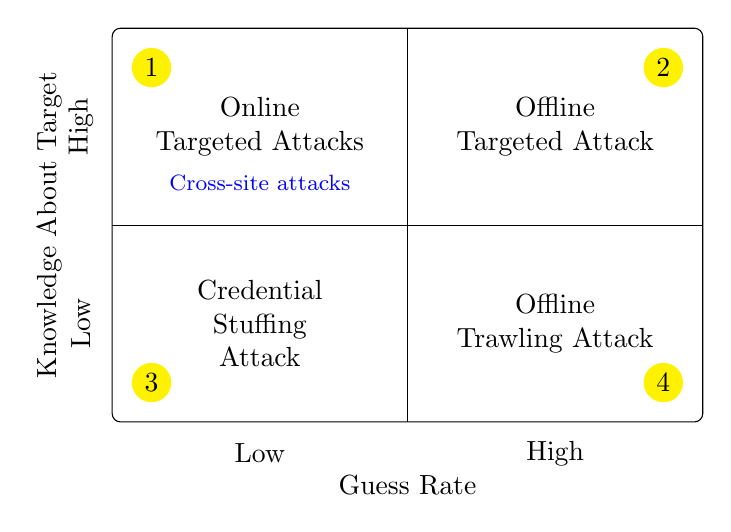
\begin{tikzpicture}
    % Variables for the grid size
    \def\gridwidth{7.5}
    \def\gridheight{5}

    % Draw the main grid
    \draw[rounded corners=3pt] (0,0) rectangle (\gridwidth,\gridheight);
    
    % Draw the dividing lines
    \draw (\gridwidth/2,0) -- (\gridwidth/2,\gridheight);
    \draw (0,\gridheight/2) -- (\gridwidth,\gridheight/2);
    
    % Labels for the attack types
    \node[align=center] (box1) at (\gridwidth/4,3*\gridheight/4) {Online\\Targeted Attacks};
    \node[align=center] at (3*\gridwidth/4,3*\gridheight/4) {Offline\\Targeted Attack};
    \node[align=center] at (\gridwidth/4,\gridheight/4) {Credential\\Stuffing\\Attack};
    \node[align=center] at (3*\gridwidth/4,\gridheight/4) {Offline\\Trawling Attack};

    \node[below, text=blue, font=\footnotesize] at (box1.south) {Cross-site attacks};
    
    % Labels for the axes
    \node[align=center] at (\gridwidth/2,-0.8) {Guess Rate};
    \node[align=center, rotate=90] at (-0.8,\gridheight/2) {Knowledge About Target};
    
    % Axis numbers
    \node[align=center] at (\gridwidth/4,-0.4) {Low};
    \node[align=center] at (3*\gridwidth/4,-0.4) {High};
    \node[align=center, rotate=90] at (-0.4,3*\gridheight/4) {High};
    \node[align=center, rotate=90] at (-0.4,\gridheight/4) {Low};


    % Circles with numbers
    % Upper left
    \node[circle,fill=yellow,inner sep=0pt,minimum size=0.5cm] at (0.5,\gridheight-0.5) {1};
    % Upper right
    \node[circle,fill=yellow,inner sep=0pt,minimum size=0.5cm] at (\gridwidth-0.5,\gridheight-0.5) {2};
    % Lower left
    \node[circle,fill=yellow,inner sep=0pt,minimum size=0.5cm] at (0.5,0.5) {3};
    % Lower right
    \node[circle,fill=yellow,inner sep=0pt,minimum size=0.5cm] at (\gridwidth-0.5,0.5) {4};

\end{tikzpicture}
\caption{Categories of attacks based on the attack rate (available to the attacker) on the horizontal axis and the amount of knowledge the attacker has about the target on the vertical axis. High attack rate signifies that the attacker has access to the target's hash. A low attack rate means that the attacker is trying to attack a hash through a rate limited service.}
\label{fig:attack-types}
\end{figure}

\begin{figure}[h]
    \centering
    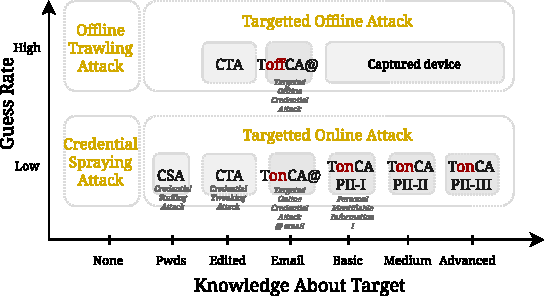
\includegraphics[scale=1.5]{figs/how_passwords/classification_of_strategy.pdf}
    \caption{Detailed representation of algorithms conditioned on guess rate and the type of information is used for targeting.}
    \label{fig::chp5::knowledge-attack-matrix}
\end{figure}

The contextual information used for targeting can be further broken down into categories that have been inspired by previous studies~\cite{pal_beyond_2019, wang_pass2edit_2023, wang_password_2023, wang_targeted_2016}. These studies have shown that using contextual information (such as previous passwords or PII) improves the likelihood of guessing human-chosen and memorable secrets. Figure~\ref{fig::chp5::knowledge-attack-matrix} visualises the detailed breakdown of contextual information with respect to the guess rate. This is summarised in Conjecture~\ref{conjecture::chp5::contextual-info}---Our analysis of the content of the password, especially the location information, showed how users embed information about themselves and environment into their secrets.

\begin{conjecture}[PII and Knowledge Embedding in Secrets]
When a person creates a secret (such as a password), they naturally embed information from their personal context into it. This embedding follows predictable patterns based on different categories of contextual information, including personal, environmental, temporal, social, and behavioural information. The likelihood of finding patterns derived from any particular type of contextual information in the secret increases with both the psychological proximity that the information has to the person and the ease with which it makes the secret memorable. This embedding occurs at a rate significantly higher than what would be expected by chance, with the strength of embedding varying based on how cognitively accessible and personally relevant the contextual information is to the creator.
\label{conjecture::chp5::contextual-info}
\end{conjecture}


\noteBox{Research Opportunity}{%
Given a limited set of strategically chosen questions about a user and their truthful answers, it is possible to generate a relatively small set of candidate passwords that contains the user's actual password with probability significantly higher than random guessing. This is achievable if and only if the questions are specifically designed to reveal information about how the user incorporates personal information into their passwords and their password creation habits. The resulting set of candidate passwords will be substantially smaller than the set of all possible passwords of the same length and character composition.
}

Conditioning a guess on assumptions about the content or structure of the password also affects guessing performance. Techniques like masking have proven highly useful in practice.

Some literature may categorise their method as a \textit{Cross-site attack}; in the context of their use, this means that the attack is targeted and uses breached passwords from other websites (hence the name cross-site). However, this strategy is often known as \textit{Credential Stuffing Attack}. If further targeting occurs, i.e., editing the password, then we call this \textit{Credential Tweaking Attack}.

Beyond credential tweaking attack, one may use more Personally Identifiable Information (PII) such as email address, date of birth, family information, and etc. As shown in Figure~\ref{fig::chp5::knowledge-attack-matrix}, we refer to these as \textbf{T}argeted \textbf{on}line \textbf{CA} (Credential Attack).

These high level strategies aim to capture the environmental limitations. There are further limitations imposed within each category, e.g. a memory-hard hash function might demand a different strategy to a simpler hash function. Also, these strategies thus far have not captured the \textit{mode} of the attack; this is the aim of the next section.

\begin{figure*}[]
    \centering
    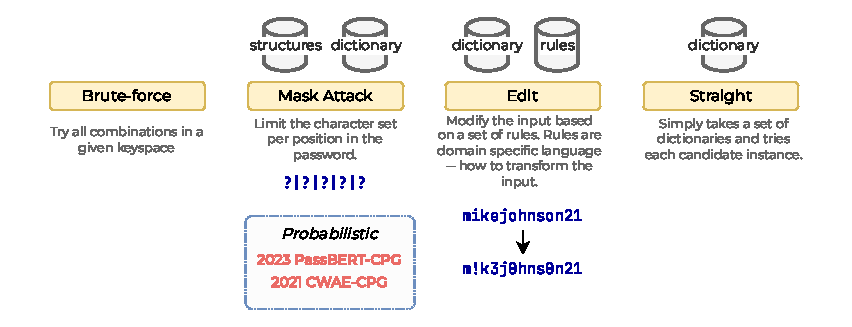
\includegraphics[scale=1.1]{figs/how_passwords/modes_passwords.pdf}
    \caption{Examples of mode of attack.}
    \label{fig::chp5::modes-of-attack}
\end{figure*}

\subsection{Generation Modes}
\label{sec::chp5::modes}

Password guessing algorithms are essentially generative functions. These algorithms can be classified into three main categories: probabilistic, deep learning-based, and deterministic (or rule-based) approaches~\cite{yu_systematic_2023, tran_survey_2022}. However, this classification is overly simplistic for practical applications. Instead, we propose categorizing password guessing algorithms based on their \textbf{mode} of attack, which better reflects their real-world effectiveness and implementation. Some of these modes are illustrated in Figure~\ref{fig::chp5::modes-of-attack}.

In academic research, most password guessing methods operate as \textit{dictionary generators}, where the primary focus is on generating potential password candidates. The actual password cracking process typically relies on established tools such as \hashcat or John the Ripper (JtR)~\cite{JtR}, which perform the hash comparison operations. These open-source tools are highly optimized to take advantage of many types of GPUs and architectures to speed up the hashing process.

\begin{definition}[Dictionary/Wordlist]
A collection of precomputed password candidates, typically containing:
\vspace{-15pt}
\begin{itemize}
\setlength{\itemsep}{-5pt}
    \item Common passwords from data breaches
    \item Words from natural languages
    \item Known password patterns
    \item Organization-specific terms
    \item Common keyboard patterns and variations
\end{itemize}
\end{definition}

The concept of attack \textbf{modes} is largely influenced by Hashcat's implementation architecture. Hashcat, together with JtR, has established itself as the industry standard for offline password cracking, offering various attack strategies optimized for different scenarios and password patterns. This mode-based approach provides a more practical framework for understanding and implementing password guessing algorithms.

\begin{itemize}
    \item \textbf{Brute-force}: In this mode, we try all combinations in a character space. This mode is essentially obsolete for any useful password guessing.
    
    \item \textbf{Mask attack}: An attacker reduces the number of combinations to try by limiting which characters can appear in each position of the password. This approach works well when the attacker knows part of the password structure. Section \ref{sec::chp5::mask-attack} explains mask attacks in detail and conducts a systemisation of the mode.
    
    \item \textbf{Edit}: An attacker modifies existing password candidates using specific rules. In Hashcat, these rules tell the programme exactly how to alter each candidate password.

    \item \textbf{Straight}: An attacker attempts passwords using a set list. \hashcat refers to this method as a \textit{Straight} attack. When attackers merge multiple dictionaries, it is termed a \textit{Combinator} attack.
    
    \item \textbf{Generative}: Attackers can generate new password candidates using several methods:
    
    \begin{itemize}
        \item \textbf{Markov n-gram models}: These analyse how frequently certain character sequences appear and use those patterns to generate likely passwords. Password crackers widely use this effective approach.
        
        \item \textbf{Probabilistic Context-Free Grammar (PCFG)}: This method creates rules on the password structure and assigns probabilities to each rule. PCFGs excel at generating passwords that look like those created by humans.
        
        \item \textbf{Deep Learning}: Networks like RNNs and GANs learn patterns from leaked password databases to generate similar passwords. As more password databases become public, researchers increasingly use deep learning to crack passwords.
        
        \item \textbf{Machine Learning}: Algorithms like decision trees, random forests, and support vector machines help attackers predict which passwords to try first.
    \end{itemize}
    
    \item \textbf{Hybrid}: An attacker combines multiple methods above to create more sophisticated attacks. For example, combine dictionary attack with mask attack.
\end{itemize}

Although these modes and password guessing attacks are presented as distinct categories, they are better approached as overlapping characteristics. For example, a generative model such as \cwaecpg using deep learning incorporates mask-like constraints. Therefore the modes and categorisations aren't mutually exclusive.

Ideally we should be able to chain these functions together and condition them on available information. The output of one function can serve as the input to another, creating a more sophisticated attack pipeline.

\subsection{Existing Algorithms}

\begin{table}[h]
%\footnotesize
\centering
\begin{tabular}{crlll}
\toprule
\textbf{Year} & \textbf{Model} & \textbf{Data} & \textbf{Comparison} & \textbf{Method} \\
\midrule
2023 & \rfguess & \begin{tabular}[c]{@{}l@{}}Rockyou\\ 000webhost\end{tabular} & \begin{tabular}[c]{@{}l@{}}FLA\\ PCFG\\ Markov\end{tabular} & \begin{tabular}[c]{@{}l@{}}Random\\ Forest Trees\end{tabular} \\
\hdashline
2022 & \gnpassgan & \begin{tabular}[c]{@{}l@{}}Rockyou\\ phpbb\end{tabular} & PassGAN & GAN \\
\hdashline
2022 & \omecdn & \begin{tabular}[c]{@{}l@{}}Rockyou\\ Yahoo\\ 12306\\ CSDN\end{tabular} & \begin{tabular}[c]{@{}l@{}}OMEN\\ PassGAN\end{tabular} & \begin{tabular}[c]{@{}l@{}}Markov\\ n-gram\end{tabular} \\
\hdashline
2021 & \adams  & 4iQ & \begin{tabular}[c]{@{}l@{}}Hashcat\\ Markov\end{tabular} & ANN \\
\hdashline
2019 & \passgan & \begin{tabular}[c]{@{}l@{}}Rockyou\\ LinkedIn\end{tabular} & \begin{tabular}[c]{@{}l@{}}Hashcat\\ PCFG\\ FLA\\ JtR\end{tabular} & GAN \\
\hdashline
2016 & \fla & \begin{tabular}[c]{@{}l@{}}PGS\\ PGS++\end{tabular} & \begin{tabular}[c]{@{}l@{}}PCFG\\ JtR\\ Hashcat\end{tabular} & LSTM \\
\hdashline
2015 & \omen & \begin{tabular}[c]{@{}l@{}}Rockyou\\ MySpace\\ Facebook\end{tabular} & \begin{tabular}[c]{@{}l@{}}Markov\\ PCFG\\ JtR\end{tabular} & \begin{tabular}[c]{@{}l@{}}Markov\\ n-gram\end{tabular} \\
\hdashline
2009 & \pcfg & \begin{tabular}[c]{@{}l@{}}MySpace\\ Finnish List\\ SilentWhisper\end{tabular} & JtR & PCFG \\
\hdashline
2005 & \markovngram & 142 Passware & Rainbow Table & \begin{tabular}[c]{@{}l@{}}Markov\\ n-gram\end{tabular} \\
\bottomrule
\end{tabular}
\caption{Examples of trawling and non-targetted password guessing methods and algorithms.}
\label{tab:password_analysis}
\end{table}


\subsubsection{PRINCE Algorithm}
The PRINCE algorithm \cite{princeprocessor2015} (\textbf{PR}obability \textbf{IN}finite \textbf{C}hained \textbf{E}lements''), is a password guessing algorithm when given an input wordlist $W$ and a target length $n$, the algorithm generates password candidates through permuted combinations. The algorithm was introduced by Jens Steube in 2014.

\subsubsection{Probabilistic Algorithms}

\textbf{Markov $\bm{n}$-gram} \cite{narayanan_fast_2005}. Markov $n$-gram models have been widely used for password guessing, with numerous iterations and improvements over time. The basic idea behind Markov $n$-gram models is to capture the statistical properties of passwords by analysing the frequency and probability of character sequences.

One notable example is \omen which outputs password guesses in descending order of their likelihood--prioritizing more probable passwords. This approach allows for more efficient password guessing by focusing on the most promising candidates first.

Building upon \omen, \omecdn incorporates a neural network-based discriminator to rank and filter the generated passwords. The discriminator, denoted as $f_{\text{GAN-D}}$, assigns a score $S$ to each password:
\begin{equation}
S = f_{\text{GAN-D}}(X)
\end{equation}
\omecdnnocite\ then selects a subset of passwords $D_{\text{OMECDN}}$ from the OMEN-generated passwords $D_{\text{OMEN}}$ based on a threshold $\gamma$:
\begin{equation}
D_{\text{OMECDN}} = { X \in D_{\text{OMEN}} : f_{\text{GAN-D}}(X) \geq \gamma }
\end{equation}
While \omecdnnocite\ provides a marginal improvement over \omennocite\ (4.07\%), it likely introduces a significant overhead in terms of generation speed compared to \omennocite.

The performance of Markov $n$-gram models can be further enhanced by incorporating additional techniques, such as smoothing and interpolation, to handle unseen or rare character sequences. Smoothing methods, such as Laplace smoothing or Kneser-Ney smoothing, assign non-zero probabilities to unseen $n$-grams, preventing the model from assigning zero probability to potentially valid passwords.

Interpolation techniques, such as linear interpolation or backoff, combine the probabilities of different order $n$-grams to improve the model's ability to handle novel sequences. For example, linear interpolation computes the probability of an $n$-gram as a weighted sum of the probabilities of lower-order $n$-grams:

% \begin{equation}
% P(x_i | x_{i-n+1}^{i-1}) = \sum_{k=1}^{n} \lambda_k P_k(x_i | x_{i-k+1}^{i-1})
% \end{equation}
% where $P_k$ denotes the probability of an $n$-gram of order $k$, and $\lambda_k$ are the interpolation weights, satisfying $\sum_{k=1}^{n} \lambda_k = 1$.

\textbf{Probabilistic Context-Free Grammar}. \pcfg\ models represent password structures as a set of grammar rules with associated probabilities. By learning the grammar from a password dataset, \pcfgnocite\ models can generate password guesses that adhere to the learned patterns and structures. The model works by dividing passwords into chunks based on letters ($L$), digits $D$, and special symbols $S$. The model then learns the rules and probabilities for these chunks from a training dataset. For example, this is how a password is represented in the \pcfgnocite\ grammar:
\[
\text{\password{password22!}} \rightarrow L_8D_2S_1
\]
Subsequent variants of the original \pcfg\ have introduced key improvements. \wordpcfg\ introduces word extraction techniques to identify semantic segments, including dictionary words, keyboard patterns, and other combinations, rather than only relying on basic character classes. \personalpcfg\ expanded the symbol sets to include semantic categories like birthdates, names, and personal information, enabling more targeted password guessing. Probability assignment has been refined by using frequency-based probabilities and non-zero probabilities for unseen strings, with some models also using cross-validation to improve generalisation. Finally, hybrid models, such as \passtcn, have been developed that integrate \pcfgnocite\ with other methods, like Markov models and Recurrent Neural Networks.

\noteBox{Research Opportunity}{%
A 2014 comprehensive review of probabilistic models by Ma et al. \cite{ma_study_2014} concludes that whole string Markov models generally outperform \pcfgnocite models in password guessing tasks. This finding suggests that capturing the statistical properties of entire passwords is more effective than modelling the underlying grammar structure. With the improvements of the original \pcfg model, and perhaps using different algorithms and architectures, it would be interesting to see whether that conclusion remains valid.
}
\vspace{-0.25cm}
\subsubsection{Deep Learning}

\fla\ was one of the first methods to use an LSTM network to model passwords and show that they can be competent and at times superior to the likes of \markovngramnocite and \pcfgnocite-based models; particularly for non-traditional password policies and when making more than $10^{10}$ guesses. Interestingly, the model did not have a material benefit from natural language dictionaries in the training set. However, an extended experiment might attempt this with different natural languages. For example, how would the results differ if the training set is in English but the test set is in Spanish?
% \fla created a larger model using c.60MB of space for offline attack and a smaller model of c.2.7MB for client-use.

\passgan\ uses a Generative Adversarial Network (GAN) to learn the distribution of real passwords from actual password leaks. Results show that it is competitive with state-of-the-art password guessing algorithms, and it can augment password generation rules by matching passwords that were not generated by other rules-based methods. There have been incremental improvements over the original \passgannocite\ model. \passgannocite\ used an Improved Wasserstein GAN (IWGAN) with gradient penalty. Subsequent models like \gnpassgan\ addressed these issues by adopting gradient normalisation on the discriminator, which imposes a gradient norm restriction, and using binary entropy loss with a sigmoid layer instead of the Wasserstein loss. This approach enhanced the discriminator's capacity, reduced mode collapse, and led to better guessing capabilities and reduced duplicate password generation.

Other improvements include changes to the network architectures. \redpack\ replaced the ResNet blocks in \passgannocite\ with Recurrent Neural Networks (RNNs), introducing a new cost function for greater stability. \gpass\ uses LSTM in the generator for better sample quality, and multiple convolutional layers with varying filter sizes in the discriminator. \gpassnocite\ also incorporates Gumbel-Softmax with temperature control, allowing for a trade-off between sample diversity and quality by adjusting the temperature during training. \cwaegan\ introduces stochastic smoothing to the password representation, which allows for more training iterations and greater model stability. The model also employs a deeper network architecture with residual bottleneck blocks and batch normalisation, which improves its ability to learn complex password patterns, leading to a higher matching rate compared to \passgannocite.

The Adaptive Dynamic Mangling rules attack (\adams) is an adaptation of Hashcat's mangling/edit mode. \adamsnocite\ aims to adapt to the target password distribution at runtime by learning best mangling rules rather than relying on static, pre-configured rules. \adamsnocite\ seems more efficient, i.e. less guesses required for a successful crack. \adamsnocite\ outperforms the standard mangling mode. Though, here the quality of the rule-set used is highly important and would have a material effect on the outcome of the experiment.

% In summary, Markov $n$-gram models have proven to be effective in password guessing tasks, with various improvements and extensions proposed over time. While PCFG models offer an alternative approach, whole string Markov models have generally demonstrated superior performance. The effectiveness of Markov $n$-gram models can be further enhanced through techniques such as smoothing and interpolation, making them a powerful tool for password guessing and security analysis.

%\textbf{RFGuess} \cite{wang_password_2023} (2023) uses Random Forest trees to generate passwords. The authors have falsely called this trawlling attack, the two algorithms sit between \textit{Credential Stuffing Attack} and \textit{Online Targeted Attack}. The authors claim that is similar to the Markov 7-gram model without much comparison to the Markov 7-gram models in the results section. They compare the model to PCFG, Markov and FLA. Experiment scenarios are split between different sites (cross-sites) and inter-site, where they use a portion of the leaked password set to the training and the remaining portion for testing. RFGuess uses the Rockyou and 000webhost dataset for the trawling attack. The results are inconclusive in our opinion. With a lack of tabular data it is difficult to judge the differences in the models. The different graphs show RFGuess performing similar to worse than its counterparts. The claim that \emph{`RFGuess outperforms all its counterparst in intra-site guessing scenarios'} can not be seen in the results. Lastly, the authors falsely claim that RFGuess is suitable for online password guessing scenarios. The results (in Fig 6 and 7 in their paper) invalidates this statement. Their claim that online guessing is unavoidable and its success is rather high is also false. Majority of websites implement rate limiting in their authentication systems. In summary, the use of Random Forest Trees for trawling attack is inconclusive from this paper and the results are deemed to be worse than their counterparts.
%
%\textbf{PassBERT} \cite{xu_improving_2023} introduces three distinct attack methodologies: Conditional Password Guessing (CPG), Targeted Password Guessing (TPG), and Adaptive Rule-based Password Guessing (ARPG). This study focuses primarily on the non-targeted trawling attack, namely CPG. The data pre-processing phase involves the exclusion of hashed passwords, the elimination of non-ASCII character passwords, and the removal of passwords exceeding 32 characters in length. Passwords undergo tokenization at the character level, incorporating the {[}CLS{]} and {[}SEP{]} tokens to signify the commencement and termination of sequences, respectively. The model's pre-training employs the Rockyou-2021 dataset, utilizing a random sampling of 60 million entries. On average, PassBERT demonstrates a password generation rate of 4.54 passwords per second. A comparative analysis is conducted with the Context Wasserstein Autoencoder (CWAE) as documented in Pasquini et al.~(2021)  \cite{pasquini_improving_2021}. Notably, the referencing of this model appears to be erroneous. The rationale provided by the authors for selecting CWAE over Pass2path (Pal et al., 2019) \cite{pal_beyond_2019} and ADaMs (Pasquini et al., 2021) \cite{pasquini_reducing_2021} is predicated on CWAE's superior performance. The reproducibility of password guessing attacks presents significant challenges. Efforts to contact the original authors for access to the model and its weights proved futile, further complicating the replication process.
%
%\textbf{CWAE} \cite{pasquini_improving_2021} This paper proposes using representation learning with deep generative models like GANs and autoencoders for password guessing. The authors train these models on leaked password datasets like RockYou to learn a latent representation of passwords that captures semantic relationships. They introduce two novel password guessing frameworks - Conditional Password Guessing (CPG) which can generate biased guesses, and Dynamic Password Guessing (DPG) which adapts the guessing strategy based on successfully guessed passwords. CPG allows generating passwords matching arbitrary templates or biases using the strong locality property of the latent space. DPG leverages the weak locality to reduce the covariate shift between train and test password distributions. The authors compare these techniques against probabilistic guessers like OMEN, PCFG and FLA on biased test sets created from LinkedIn data. They show CPG can efficiently generate rare biased guesses unlike other methods. DPG adapts and outperforms static attacks on diverse leaks like Youku and Zomato exhibiting distribution shifts.

%\textbf{PASS2EDIT} (2023) \cite{wang_pass2edit_2023} introduces a new approach for guessing edited passwords in targeted attacks by modelling password tweaking as a multi-class classification problem. The authors propose a multi-step decision-making mechanism combined with a generative model to characterize users' password reuse and modification behaviours. They evaluate PASS 2 EDIT using 12 attack scenarios and a large dataset of 4.8 billion passwords.
%The paper claims that PASS 2 EDIT outperforms prior methods such as Pass2Path and TarGuess-II, achieving 18.2\%-33.0\% higher cracking success rates within 100 guesses when the victim's password at one site is known. However, the evaluation relies heavily on the specific attack scenarios and datasets chosen, and the generalizability of the results to other settings is unclear.
%While the authors emphasize the severity of password tweaking threats, the practical impact may be less significant than suggested, as the success rates are still relatively low even with PASS 2 EDIT. Moreover, the paper does not adequately address the limitations of the proposed approach or discuss potential countermeasures.
%Overall, PASS2EDIT offers a new perspective on characterizing password reuse behaviours but falls short of providing a comprehensive understanding of users' password security. The claims of superiority over prior art should be interpreted with caution, as the evaluation is limited in scope and may not reflect real-world performance in diverse settings.

\subsection{Limitations of Existing Methods}
Current methods do not incorporate the speed of generation, which is an important factor that most open-source tools and industry have focused on. We believe a practical method would factor in both generation speed and quality of output, i.e. the number of guesses. The next station aims to model the password guessing process and incorporate these two factors to determine the true practical performance.

\section{Process}
\label{sec::chp5::process}

\begin{figure}[t]
\centering
\begin{tikzpicture}[
node distance=3.5cm,
block/.style={rectangle, rounded corners, draw, minimum width=2cm, minimum height=1.5cm},
queue/.style={rectangle, rounded corners, draw, minimum width=1cm, minimum height=0.8cm},
arrow/.style={->, thick}
]
% Generation stage
\node[block] (gen) {Password Generation};
% Queue
\node[queue, right of=gen] (queue) {Queue};
% Hashing stage
\node[block, right of=queue] (hash) {Hashing $\mu$};
% System boundary
\draw[dashed] ($(gen.north west)+(-0.2,0.2)$) rectangle ($(hash.south east)+(0.2,-0.2)$);
% Arrows
\draw[arrow] ($(gen.east)$) -- node[above] {$\lambda$} (queue.west);
\draw[arrow] (queue.east) -- node[above] {} (hash.west);
% System parameters
\node[below=0.8cm of queue] {System Utilization $\rho = \frac{\lambda}{\mu}$};
% Labels
\node[above=0.4cm of gen] {Stage 1};
\node[above=0.4cm of hash] {Stage 2};
% Optional explanation
% \node[below=1.5cm of hash, align=left, text width=20cm] 
%     {$\lambda$: Password candidate generation rate\\
%      $\mu$: Hash computation rate\\
%      $\rho$: System utilization};
\end{tikzpicture}
\caption{Visual representation of the password guessing process. Assuming an offline scenario where the attacker posses the hash value. $\lambda$ is password generation rate and arrival rate; $\mu$ is the hash rate or service rate; and $\rho$ is the utilization rate of the system.}
\label{fig:password-guessing-model}
\end{figure}

When attackers attempt to guess passwords, they must overcome hash functions that are designed to be computationally infeasible to invert (one-way function property). Therefore, we should naturally be interested in the rate at which they attempt this guessing. Whilst industry and the open-source community have focused on optimising hash rates to traverse the search space more quickly, academic literature and models have conversely neglected such optimisation. The question for us then is whether the newly proposed models perform better than even brute-force methods.

Systematising the guessing process provides a framework for optimising and allocating resources efficiently. By identifying bottlenecks, such as a slow dictionary generator, we can compare and select algorithms based on specific scenarios. Each stage in the process requires different resources, such as GPUs; therefore, modelling this process enables us to allocate these resources effectively. This systematic approach allows us to determine precisely how and when to scale or parallelise resources. Moreover, such a model helps to accurately determine both the cost and the time requirements for the entire process.

We model the password guessing process in two distinct steps: 1) Generation: This step produces a potential candidate for a given hash, and 2) Hashing: in this step, we compute the hash of the candidate password produced in the previous step. Whilst we assume that we are carrying out an offline attack (where we possess the hash value), this model can be generalised for other modes of attack. This process is visualised in Figure~\ref{fig:password-guessing-model}.

% \begin{axiom}[Offline Attack Assumption]
% Given a target hash value $h_t \in \{0,1\}^n$, the attacker has unrestricted access to $h_t$ and can compute $H(p)$ for any $p \in \mathcal{P}$.
% \end{axiom}
% 
% \begin{definition}[Password Guessing Process]
% Let $\mathcal{P}$ be the space of all possible passwords and $h: \mathcal{P} \rightarrow \{0,1\}^n$ be a cryptographic hash function. A password guessing process is a tuple $(G, H)$ where:
% \begin{itemize}
%     \item $G: \mathbb{N} \rightarrow \mathcal{P}$ is a generation function that produces candidate passwords
%     \item $H: \mathcal{P} \rightarrow \{0,1\}^n$ is the hash computation function
% \end{itemize}
% \end{definition}


%\begin{theorem}[Optimization Framework]
%The password guessing optimization problem can be formulated as:
%
%\[\min_{G} \{\mathbb{E}[X] \cdot \mathbb{E}[T]\}\]
%
%where $T$ is the random variable representing the time to generate and hash a single guess, subject to:
%\begin{enumerate}
%    \item $G$ must be computationally feasible
%    \item $\forall p \in \mathcal{P}, \exists i \in \mathbb{N}: G(i) = p$ (completeness)
%\end{enumerate}
%\end{theorem}
%
%\begin{definition}[Search Space Reduction]
%The efficiency of a generation function $G$ can be quantified by the search space reduction ratio:
%
%\[\rho(G) = \frac{|\{G(i): i \leq \mathbb{E}[X]\}|}{|\mathcal{P}|}\]
%
%where $\rho(G) \in (0,1]$ represents the fraction of the password space that must be explored before finding the target.
%\end{definition}


To optimise a password guessing algorithm, we need to balance two key factors:
\vspace*{-0.5cm}
\begin{enumerate}
    \item How well the algorithm guesses---measured by how many guesses it needs before succeeding. We can express this as $\mathbb{E}[X]$, where X represents the number of guesses.
    \vspace{-0.25cm}
    \item How quickly the algorithm generates its guesses. We measure this speed using $N(t)$, which represents the total guesses the algorithm has made by time t.
\end{enumerate}
% \begin{definition}[Guessing Efficiency]
% For a target password $p_t \in \mathcal{P}$ with hash $h_t = h(p_t)$, we define:
% \begin{itemize}
%     \item The number of guesses until success: $X = \min\{i: H(G(i)) = h_t\}$
%     \item The expected number of guesses: $\mathbb{E}[X]$
%     \item The guessing rate function: $N: \mathbb{R}^+ \rightarrow \mathbb{N}$, where $N(t)$ represents the cumulative number of guesses made by time $t$
% \end{itemize}
% \end{definition}

\subsection{Password Guessing Probability}

We will now incorporate the probability of successful guesses after a $x$ number of guesses guesses. Let $F(x)$ be the cumulative probability distribution function (CDF) of successful password guesses after $x$ number of guesses. $F(x)$ is essentially an assumed distribution by a guessing algorithm and we are interested in comparing these assumed distributions against each other with the ultimate aim of incorporating time (more on this in Section~\ref{how-passwords::time-to-crack}.)

\paragraph{Brute-force:}

The base case is a brute-force method that can be modelled using a uniform distribution. Let us assume the length of character space is $C$ and the length of a password is $\ell$. Our search space would therefore be $C^\ell$.

Uniform distribution for the brute-force method becomes:
\begin{equation}
    F_{\ell}(x) = \min \Bigl\{ \frac{x}{C^\ell},\,1 \Bigl\}
\end{equation}

Let $\mathcal{L}: \Omega \to \{1,\ldots,n\}$ be the random variable length. The composite distribution function becomes:

\begin{equation}
F_B(x) = \sum_{\ell=1}^n F_\ell(x) \, \mu_{\mathcal{L}}(\ell)
\end{equation}

where $\mu_{\mathcal{L}}$ is the probability mass function of password lengths. This then resolves to:

\begin{equation}
F_B(x) = \sum_{\ell=1}^n \min \Bigl\{ \frac{x}{C^\ell},\,1 \Bigl\} \, \mu_{\mathcal{L}}(\ell)
\end{equation}

% TODO: duplicated passwords
% Let $H = \{h_1, ..., h_k\}$ be a set of salted password hashes and $\mu_L: \mathbb{N} \to [0,1]$ be a password length distribution. The cumulative probability distribution function is:
% 
% $$
% F_B(x) = 1 - \prod_{i=1}^k \left(1 - \sum_{\ell \in \mathbb{N}} \min\left\{\frac{x}{C^\ell}, 1\right\} \mu_L(\ell)\right)
% $$
% 
% Taking the logarithm:
% 
% $$
% \log(1 - F_B(x)) = k \log\left(1 - \sum_{\ell \in \mathbb{N}} \min\left\{\frac{x}{C^\ell}, 1\right\} \mu_L(\ell)\right)
% $$
% 
% The expected number of guesses:
% 
% $$
% E[X] = \int_0^\infty \left(1 - \sum_{\ell \in \mathbb{N}} \min\left\{\frac{x}{C^\ell}, 1\right\} \mu_L(\ell)\right)^k dx
% $$
% 
% where:
% \begin{align*}
% k &: \text{number of salted hashes} \\
% C &: \text{character space size} \\
% \mu_L(\ell) &: \text{probability of length } \ell \\
% \sum_{\ell \in \mathbb{N}} \mu_L(\ell) &= 1
% \end{align*}

\paragraph{Logistic function:}

Based on the empirical results (as we shall see in Section~\ref{how-passwords::empirical-eval}), the deep learning models fit a logistic function well.
\begin{equation}
    F_L(x) = \frac{M}{1 + e^{-k(x-x_0)}}
\end{equation}
Where:
\begin{align*}
M & : \text{ maximum asymptotic value} \\
k & : \text{ logistic growth rate coefficient} \\
x_0  & : \text{ horizontal shift parameter (inflection point)} \\
\end{align*}

% \begin{equation}
% F(x) = 1 - e^{-(x/\eta)^\beta}
% \end{equation}
% \begin{equation}
% F(x) = A\,( 1 - e^{-bx} )
% \end{equation}
% where $\eta$ is the scale parameter and $\beta$ is the shape parameter.

\begin{figure}[t]
    \centering
    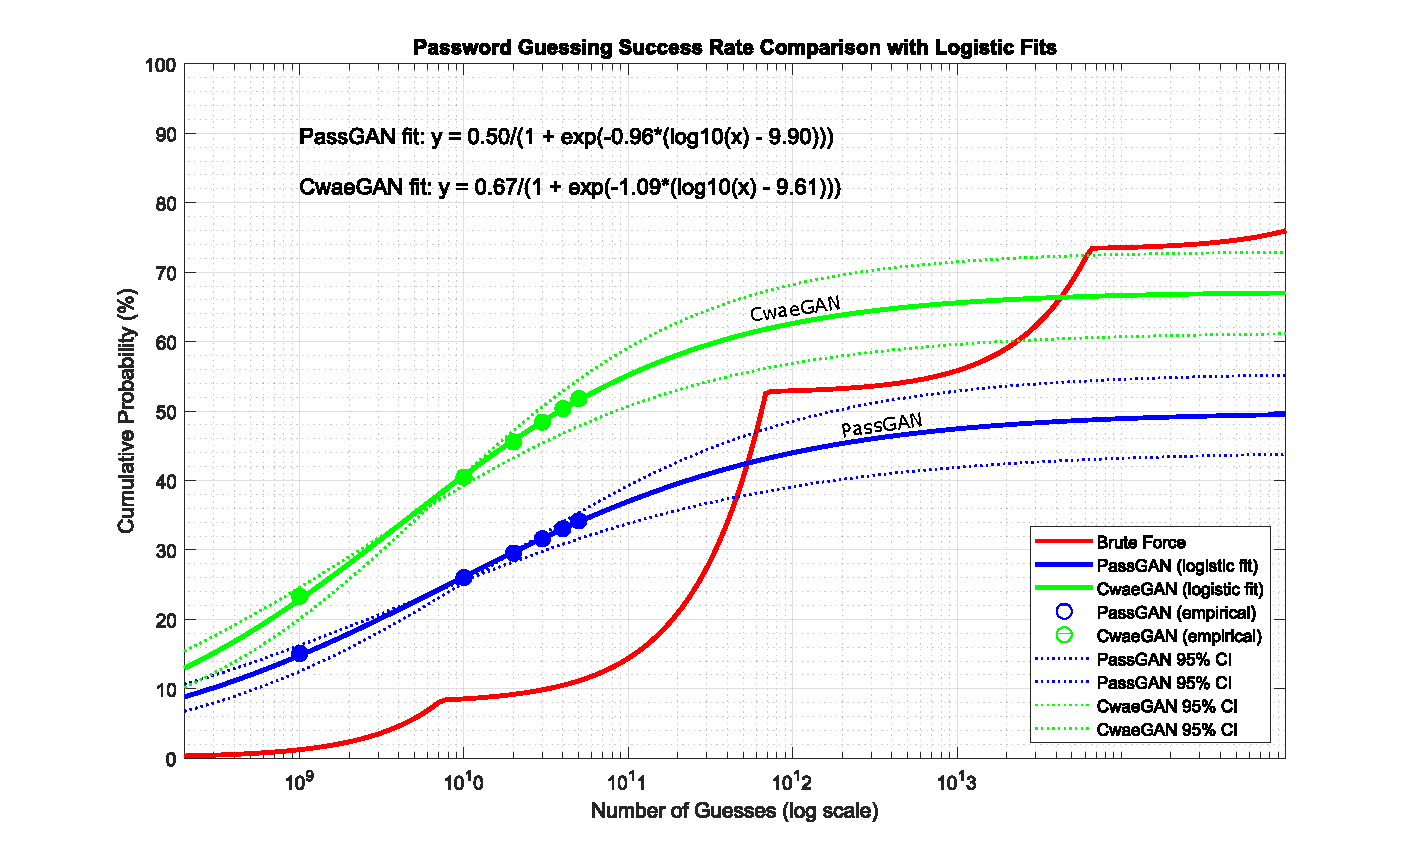
\includegraphics[scale=0.6]{figs/how_passwords/expected_guesses_chart2.pdf}
    \caption{Chart showing the cumulative probability distribution of \passgan, a similar GAN model (\cwaegan) and a brute-force method based on the Rockyou length distribution. The data fro the GAN models are taken from the same experiment and fitted with a logistic function. \srcOwnFig}
    \label{fig:password-expected-guesses}
\end{figure}

\subsection{Number of Guesses Empirical Evaluation}
\label{how-passwords::empirical-eval}

Putting our theoretical work into practice to this point, we want to ask how well the algorithms perform compared to the brute-force method. For this, we select the trawling attacks described in the \cwaegan and \omecdn papers.

For the length distribution $\mu_{\mathcal{L}}(\ell)$ (in brute-force method) we will use the empirical distribution from the Rockyou dataset as both papers used the RockYou password leak for training and testing their models, though they reported dataset details quite differently. The \omecdn paper provided comprehensive statistics, stating they used the Skullsecurity RockYou leak containing 32.6M passwords, which reduced to 14.3M after deduplication, and was further processed by removing passwords over 10 characters and those with illegal characters before being split 80:20 for training and testing. In contrast, the \cwaegan paper only briefly mentioned using the RockYou corpus with passwords up to 10 characters and filtered uncommon characters, but did not provide specific dataset sizes or train/test split details. This difference in dataset transparency makes it difficult to directly compare model performance.

We assume that models stop producing meaningful password candidates at some point and therefore the logistic function fits the empirical data well--as shown in Figure \ref{fig:password-expected-guesses}. The brute-force method overtakes the two GAN models in \cwaegan\ at $\sim4.7\times10^{13}$ guesses (68\% successful guesses). 
%%%%%%%%%%%%%%%%%%%%%%%%%%%%%%%%%%%%%%%%%%%%%%%%%%%%%%%%%%%%%%%%
\subsection{Expected Time to Crack}
\label{how-passwords::time-to-crack}
Let's assume the cumulative number of guesses made up to time $t$ is $N(t)$, therefore the cumulative probability of a successful guess by time $t$ is $F(N(t))$.  With this we can proceed to modelling the expected time to crack a password.
\begin{equation}
N(t) = \min(\lambda,\,\mu)\,t
\end{equation}
The system's performance metric combines both the queueing dynamics and success probability. The probability that the password is found in the interval $[t, t + dt]$ is $dF(N(t))$, so the expected time is:
\begin{equation}
\mathbb{E}[T_c] = \int_0^\infty t\,\frac{d}{dt}F(N(t))\,\di t = \int_0^\infty t\,f(N(t))\,N'(t)\,\di t
\end{equation}
To compute the expected time to successfully guess a password, we consider the time until a successful guess occurs, which depends on the number of processed guesses and their success probabilities. $N'(t) = \frac{dN(t)}{dt}$ is the rate at which the guesses are processed.

\paragraph{Uniform/Brute-force Function:}

\begin{multline*}
\\
\text{Starting with our CDF for brute-force:} \\
F_B(x) = \sum_{\ell=1}^n \min \Bigl\{ \frac{x}{C^\ell},\,1 \Bigr\} \, \mu_{\mathcal{L}}(\ell) \\
\end{multline*}
Evaluating the function with $N(t) = \min(\lambda, \mu)t$:
\begin{equation}
F_B(\min(\lambda, \mu)t) = \sum_{\ell=1}^n \min \Bigl\{ \frac{\min(\lambda, \mu)t}{C^\ell},\,1 \Bigr\} \, \mu_{\mathcal{L}}(\ell)
\end{equation}
This equation identifies the critical point where the ratio equals unity, representing the threshold condition for level $\ell$.
\begin{equation}
\frac{\min(\lambda, \mu)t}{C^\ell} = 1
\end{equation}
We define $T_\ell$ as the ratio of capacity at level $\ell$ to the minimum rate. This represents the time required to reach capacity at each level.
\begin{equation}
T_\ell = \frac{C^\ell}{\min(\lambda, \mu)}
\end{equation}
Substituting back:
\begin{equation}
\mathbb{E}[T_c] = \sum_{\ell=1}^n \mu_{\mathcal{L}}(\ell) \cdot T_\ell
\end{equation}
Finally:
\begin{equation}
\mathbb{E}[T_c] = \frac{1}{\min(\lambda, \mu)} \sum_{\ell=1}^n C^\ell \mu_{\mathcal{L}}(\ell)
\end{equation}

\paragraph{Logistic Function:}

Calculating the probability density function for our logistic CDF:
\begin{equation*}
F_L(x) = \frac{M}{1 + e^{-k(x-x_0)}}
\end{equation*}
\begin{equation*}
\text{Let } u = -k(x-x_0)
\end{equation*}
Substituting to simplify differentiation and using the chain rule:
\begin{equation*}
F(x) = M(1 + e^u)^{-1}
\end{equation*}
\begin{equation*}
\frac{dF}{du} = M \cdot (-1)(1 + e^u)^{-2} \cdot e^u
\end{equation*}
\begin{equation*}
\frac{du}{dx} = -k
\end{equation*}
Multiplying the derivatives:
\begin{equation*}
\frac{dF}{dx} = M \cdot (-1)(1 + e^u)^{-2} \cdot e^u \cdot (-k)
\end{equation*}
Simplifying:
\begin{equation*}
\frac{dF}{dx} = Mk \cdot \frac{e^u}{(1 + e^u)^2}
\end{equation*}
Final probability density function:
\begin{equation}
f_L(x) = Mk \cdot \frac{e^{-k(x-x_0)}}{(1 + e^{-k(x-x_0)})^2}
\end{equation}

\begin{figure}[ht]
    \centering
    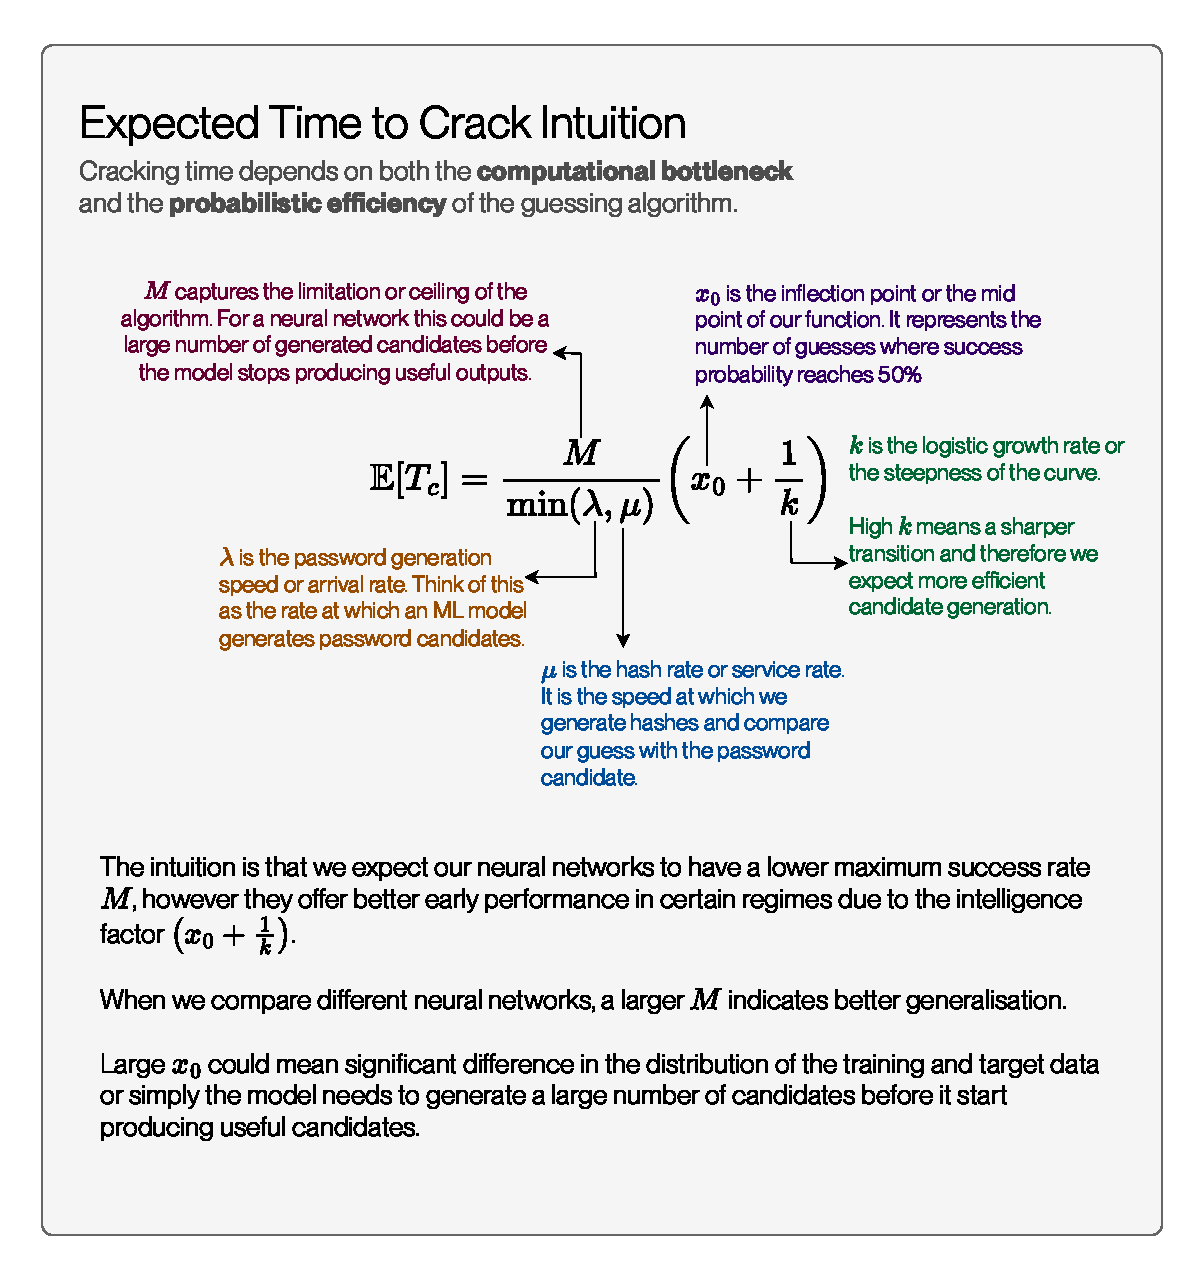
\includegraphics[width=0.7\linewidth]{figs//how_passwords/phd_equation.pdf}
    \caption{Visualisation of Equation~\ref{eq::515}. This figure explains the variables and provides some intuition behind the equation.}
    \label{fig::chp5::e_t_crack}
\end{figure}

Now we can calculate the expected Time to Crack for our logistic function:
\begin{align*}
\mathbb{E}[T_c] & = \int_0^\infty t \cdot \frac{kM\alpha e^{-k(\alpha t - x_0)}}{(1 + e^{-k(\alpha t - x_0)})^2}\,dt \\
& = \int_{-x_0}^\infty \frac{u + x_0}{\alpha} \cdot \frac{kM\alpha e^{-ku}}{(1 + e^{-ku})^2} \cdot \frac{du}{\alpha} \\
& = M\int_{-x_0}^\infty \frac{(u + x_0)ke^{-ku}}{(1 + e^{-ku})^2}\,du \\
& = M\left[\frac{x_0}{\alpha} + \frac{1}{k\alpha}\right] \\
\end{align*}
Our final equation then becomes:
\begin{equation}
\mathbb{E}[T_c] = \frac{M}{\min(\lambda, \mu)}\left(x_0 + \frac{1}{k}\right)
\label{eq::515}
\end{equation}

Equation~\ref{eq::515} shows the expected time to crack a password. $\lambda$ represents our arrival rate (or the number of password guesses we generate using a model), whilst $\mu$ is the hashing rate (or how many password hashes we can generate per unit of time). So, $\min(\lambda, \mu)$ tells us by what our system is throttled and is the \textit{effective} password guessing rate. Together, the expression $\left(x_0 + \frac{1}{k}\right)$ scales the basic time estimate $\frac{M}{\min(\lambda, \mu)}$ to account for both initial search conditions and the probabilistic nature of password discovery. This gives us a more realistic expected completion time that reflects both the computational constraints and the stochastic aspects of the guessing process. Figure~\ref{fig::chp5::e_t_crack} provides a detailed breakdown of the equation in visual form.

% TODO: Weibull distribution for expected guesses.
%\paragraph{Weibull distribution:}
%
%Substituting $f(N(t))$ and $N'(t)$, we get:
%\[
%E[T] = \int_0^\infty t \, \frac{\beta}{\eta} \left( \frac{N(t)}{\eta} \right)^{\beta - 1} e^{-(N(t)/\eta)^\beta} N'(t) \, dt.
%\]
%
%In cases where $N(t) = \nu t$, with $\nu = \min\{\lambda, \mu\}$, we have $N'(t) = \nu$, and $N(t) = \nu t$, so:
%\[
%E[T] = \int_0^\infty t \, \frac{\beta \nu^\beta}{\eta^\beta} t^{\beta - 1} e^{-(\nu t / \eta)^\beta} dt.
%\]
%
%Simplifying:
%\[
%E[T] = \frac{\beta \nu^\beta}{\eta^\beta} \int_0^\infty t^\beta e^{-(\nu t / \eta)^\beta} dt.
%\]
%
%Letting $u = \left( \frac{\nu t}{\eta} \right)^\beta$, we have:
%\[
%t = \frac{\eta}{\nu} u^{1/\beta}, \quad dt = \frac{\eta}{\nu} \frac{1}{\beta} u^{(1/\beta) - 1} du.
%\]
%
%Substituting back, we get:
%\[
%E[T] = \frac{\beta \nu^\beta}{\eta^\beta} \cdot \frac{\eta}{\nu} \cdot \frac{1}{\beta} \int_0^\infty \left( \frac{\eta}{\nu} u^{1/\beta} \right)^\beta u^{(1/\beta) - 1} e^{-u} du.
%\]
%
%Simplifying, the integrand becomes:
%\[
%\left( \frac{\eta}{\nu} u^{1/\beta} \right)^\beta = \left( \frac{\eta}{\nu} \right)^\beta u.
%\]
%
%Therefore, the expected time simplifies to:
%\[
%E[T] = \frac{\nu^\beta}{\eta^\beta} \cdot \frac{\eta}{\nu} \cdot \left( \frac{\eta}{\nu} \right)^\beta \int_0^\infty u e^{-u} du = \frac{\eta}{\nu} \Gamma(2),
%\]
%where $\Gamma(2) = 1! = 1$.
%
%Thus, the expected time to find the password is:
%\[
%E[T] = \frac{\eta}{\nu}.
%\]
%
%However, this result holds for $\beta = 1$, which corresponds to the exponential distribution. For a general $\beta$, the expected number of guesses is:
%\[
%E[N] = \eta \Gamma\left(1 + \frac{1}{\beta}\right),
%\]
%so the expected time to find the password is:
%\[
%E[T] = \frac{E[N]}{\nu} = \frac{\eta}{\nu} \Gamma\left(1 + \frac{1}{\beta}\right).
%\]
\subsection{Time to Crack Empirical Evaluation} 

\begin{figure}
    \centering
    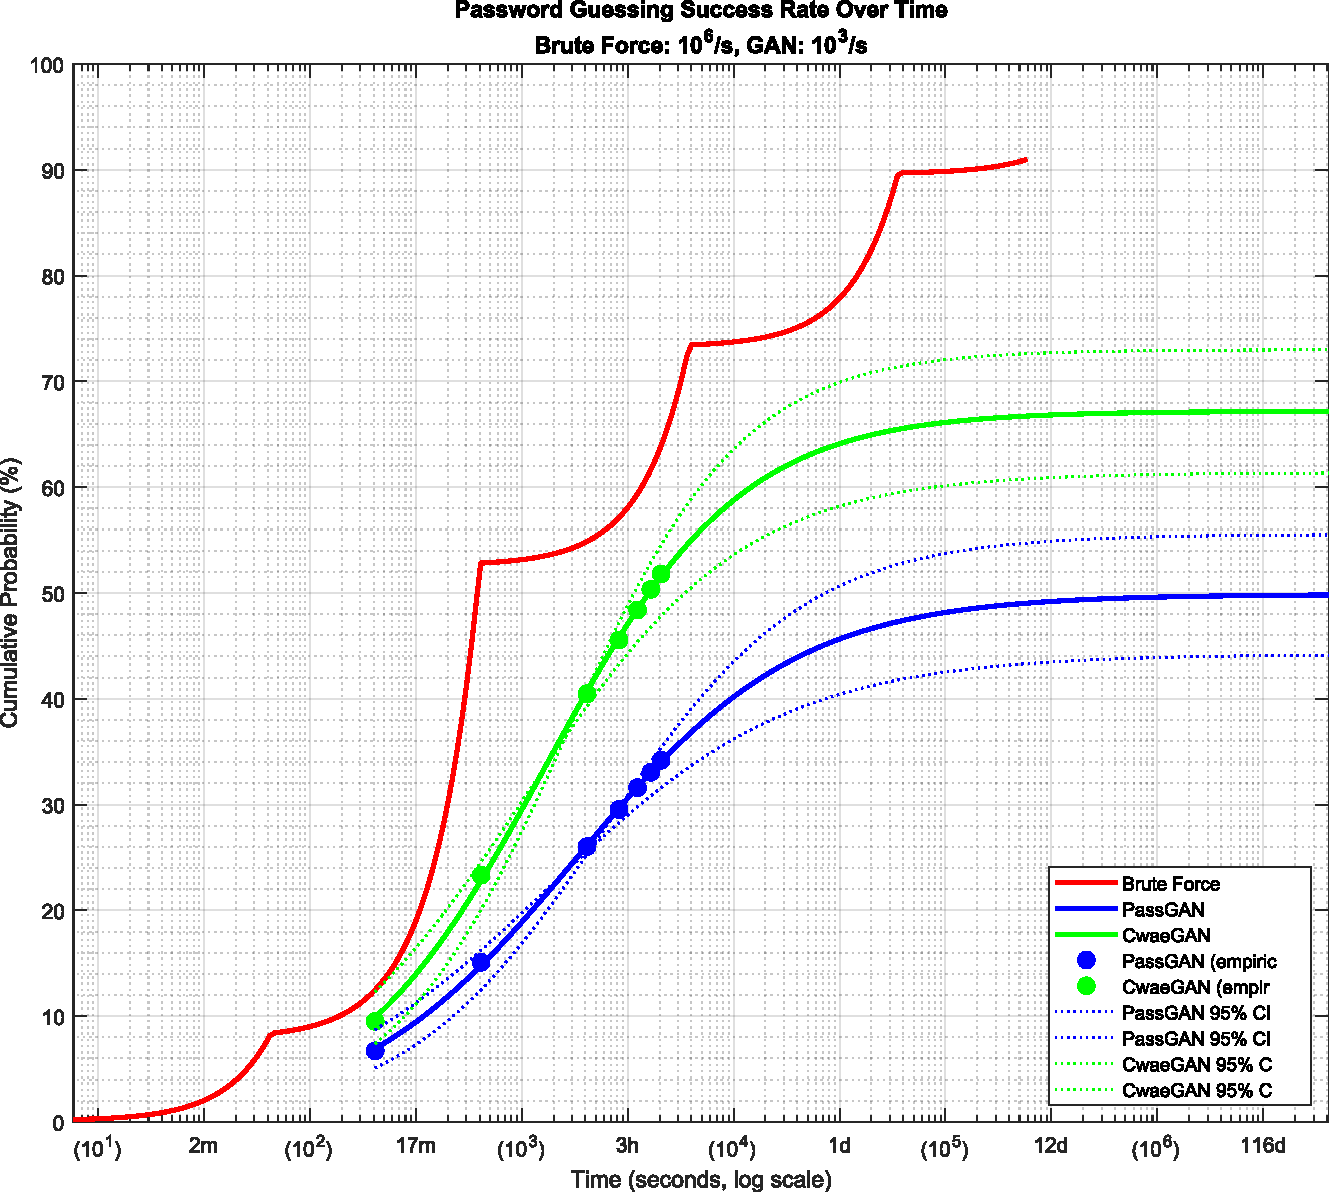
\includegraphics[scale=0.6]{figs/how_passwords/time_cdf.pdf}
    \caption{Calculating $F(N(t))$, incorporating both probability of guessing and the rate at which it happens gives us a more accurate view of the performance of password guessing algorithms. This framework demonstrates the utility of considering both generation quality and speed. \srcOwnFig}
    \label{fig:cracking-time}
\end{figure}

Figure~\ref{fig:cracking-time} shows our result using the same models as the number of guesses section. Here we assume the process is throttled by the number of candidates the GAN models are generating, i.e. $N(t) = \lambda t$, where $\lambda$ is the arrival rate and therefore the generation speed.

For our empirical analysis, we used the same dataset configurations as in the previous guessing probability evaluation - the RockYou password leak processed to contain passwords up to 10 characters. We measured the actual time taken to generate and process password guesses using both brute-force and GAN approaches across different hardware configurations.

The hashing rate $\mu$ is based on \hashcat benchmarks on consumer-level hardware. The hash rate is dependent on the hash function we are inverting and the hardware being used. Higher hash rate favours the brute-force method.

% \begin{enumerate}
% \item Despite lower raw generation rates, GAN models initially achieve faster crack times for common passwords due to their more intelligent probability distribution of guesses.
% \item For passwords beyond the 60th percentile of complexity, the brute-force method becomes more efficient due to its superior generation rate overwhelming the GANs' more targeted guessing strategy.
% \item The crossover point occurs at approximately 45 minutes of cracking time on our test hardware, after which brute-force methods consistently outperform the GAN approaches.
% \end{enumerate}

This empirical analysis supports our theoretical predictions about the relationship between generation rate, hash rate, and cracking success. It also highlights an important practical consideration: while sophisticated guessing strategies may be more efficient for common passwords, hardware-optimized can remain competitive and optimisation of the implementations should be considered a novel piece of work.

\subsection{Other Strategies and Parallelisation}

In the two-stage model considered in this chapter (candidate generation \(\rightarrow\) hash verification), the effective cracking throughput is determined by the bottleneck between the candidate generation rate \(\lambda\) and the hash-processing capability \(\mu\). Here, the application of more advanced queueing theory would be beneficial for understanding how scaling the number of workers would affect guessing rates. Moreover, future work could also incorporate cost and the economics of password guessing at scale. In Figures~\ref{fig:cracking-time}~and~\ref{fig:password-expected-guesses}, we assumed the attacker is not parallelising either \(\lambda\) or \(\mu\). The attacks are conducted on a consumer level hardware (internally the hashing might be parallelised at CPU or GPU level).

Increasing the number of generator or hashing workers changes the arrival process \(N(t)\) and consequently the expected time-to-crack derived earlier. Framing parallelism in this way allows formal comparison between algorithmic improvements (better candidate ranking) and systems improvements (higher \(\lambda\) or \(\mu\)).

For neural-network-based attacks, the system becomes constrained by the model’s candidate-generation rate rather than by the computational hashing throughput. Generating intelligent password candidates requires significantly more computational resources per guess than verifying them. In this scenario, we can scale the number of generators, optimise generation speed through model compression or quantisation techniques, or precompute candidates. Ultimately, the strategy to choose depends on the attacker’s intent, the type of neural network, and the target. There are leaked password dictionaries with billions of records already, so unless the neural network has better or more novel candidates, precomputing may not be useful.

When scaling the candidate-generation workers for neural networks, we can theoretically match or exceed the hashing rate $\mu$, but this approach faces practical limitations due to memory-bandwidth constraints, inter-processor communication overheads, and the inherently sequential nature of some neural network operations. However, parallelisation enables neural networks to reach their maximum potential, $M$, more quickly, without fundamentally altering their learning characteristics. Therefore, we would merely reach that asymptotic ceiling more quickly while preserving the underlying intelligence limitations of the model architecture.

For naive brute-force strategies, the hashing rate can be parallelised almost linearly, significantly improving $\mu$. This near-perfect parallel scaling gives brute-force approaches a significant advantage in highly parallel environments, potentially offsetting some of the intelligence-related benefits of neural approaches when sufficient computational resources are available.

Our work in this section remains valid when applying parallelisation techniques, and the approach we have taken enables us to reason effectively about parallelisation. Moreover, it prepares us to carry out future experiments using queueing theory, and even to consider the economics of password-guessing strategies.

% %\subsection{Queueing Model}
We model the process using a single server queue. The potential candidates are generated at near deterministic rate $\lambda$ and similarly the passwords are hashed and processed at near deterministic rate $\mu$. Therefore using Kendal's notation, the system is modelled as G/G/1. Let $\lambda(t)$ represent the arrival rate, and let $\mu(t)$ represent the hashing rate (this is typically referred to as the service rate). The utilization of our hashing server $H$ is:
\begin{equation}
    \rho = \frac{\lambda}{\mu}
\end{equation}

The utilization factor $\rho = \frac{\lambda}{\mu}$ must satisfy $\rho < 1$ for system stability, implying that the generation rate cannot exceed the processing capacity of the hashing function. 

\[
\rho = \lambda \, \mathbb{E}[S]
\]

The expected wait time in the system (queue and hashing) is given by the Kingman's approximation for our G/G/1 system.
\begin{equation}
    \mathbb{E}[W] = \frac{\rho}{1 - \rho} \cdot \frac{c_a^2 - c_s^2}{2} \cdot \mathbb{E}[S]
\end{equation}
The expected time in the system for a given password candidate:
\begin{equation}
    \mathbb{E}[T] = \mathbb{E}[S] + \mathbb{E}[W]
\end{equation}
\begin{equation}
    \mathbb{E}[T] = \left[ 1 + \frac{\rho}{1 - \rho} \cdot \frac{c_a^2 - c_s^2}{2} \right] \cdot \mathbb{E}[S]
\end{equation}
Based on, we can now calculate the expected number of password candidates in the system using Little's law:
\begin{equation}
    \mathbb{E}[N] = \lambda \mathbb{E}[T]
\end{equation}
\begin{equation}
    \mathbb{E}[N] = \rho + \frac{\rho^2(c_a^2 - c_s^2)}{2(1 - \rho)}
\end{equation}

Ideally we would like our server to be operating at maximum capacity, i.e. to maximise the resources available. This implies that our password generation should match the service rate of our server. However, we still want password candidates with high probability of inverting the hash function. So, a better measure of password guessing algorithm would be the expected time to crack--i.e. the expected time for an algorithm to invert the hash function. This takes into consideration the resources available to us and the probability distribution of an algorithm successfully guessing a password.

% \subsection{Resource Constraints and Optimization}
% 
% Let $C(t)$ represent the computational cost function:
% \[
% C(t) = c_g \int_0^t \lambda(s) \, ds + c_h \int_0^t \min\{\lambda(s), \mu(s)\} \, ds,
% \]
% where $c_g$ and $c_h$ are the unit costs for candidate generation and hashing, respectively.
% 
% The optimization problem can be formulated as:
% \begin{align*}
% \max_{\lambda(t)} & \quad F(N(T)) \\
% \text{subject to:} & \quad C(T) \leq B, \\
% & \quad \lambda(t) \geq 0, \\
% & \quad \int_0^T \lambda(t) \, dt \leq K,
% \end{align*}
% where $B$ represents the total computational budget and $K$ is the maximum number of allowable guesses.
% 
% To solve this optimization problem, we set up the Lagrangian:
% \[
% \mathcal{L} = F(N(T)) - \alpha \left( C(T) - B \right) - \gamma \left( \int_0^T \lambda(t) \, dt - K \right),
% \]
% where $\alpha \geq 0$ and $\gamma \geq 0$ are Lagrange multipliers.
% 
% Taking the functional derivative of $\mathcal{L}$ with respect to $\lambda(t)$, we obtain the necessary condition for optimality:
% \[
% \frac{\delta \mathcal{L}}{\delta \lambda(t)} = \frac{dF}{dN} \frac{dN}{d\lambda(t)} - \alpha \left( c_g + c_h \frac{d}{d\lambda(t)} \min\{\lambda(t), \mu(t)\} \right) - \gamma = 0.
% \]
% 
% The derivative $\frac{dN}{d\lambda(t)}$ depends on whether $\lambda(t) \leq \mu(t)$ or $\lambda(t) > \mu(t)$.
% 
% If $\lambda(t) < \mu(t)$:
% \[
% \min\{\lambda(t), \mu(t)\} = \lambda(t), \quad \frac{d}{d\lambda(t)} \min\{\lambda(t), \mu(t)\} = 1,
% \]
% so the derivative simplifies.
% 
% If $\lambda(t) > \mu(t)$:
% \[
% \min\{\lambda(t), \mu(t)\} = \mu(t), \quad \frac{d}{d\lambda(t)} \min\{\lambda(t), \mu(t)\} = 0.
% \]
% 
% Therefore, we need to consider these cases separately to derive the optimal control for $\lambda(t)$.

% \subsection*{Weibull Parameter Estimation}
% 
% Empirical studies, such as those involving PassGAN, have shown that password success probabilities can be approximated by the Weibull distribution. Given a success rate $p$ after $n$ guesses, the Weibull parameters can be determined by solving:
% \[
% p = F(n) = 1 - e^{-(n/\eta)^\beta}.
% \]
% 
% Taking the natural logarithm of both sides:
% \[
% \ln(1 - p) = -\left( \frac{n}{\eta} \right)^\beta.
% \]
% 
% Taking the logarithm again:
% \[
% \ln(-\ln(1 - p)) = \beta \ln n - \beta \ln \eta.
% \]
% 
% This linear relationship allows for estimation of $\beta$ and $\eta$ using linear regression on the transformed data, plotting $\ln(-\ln(1 - p))$ versus $\ln n$.



% \begin{itemize}[leftmargin=11pt]
% \item \textbf{\textsc{Generate.}} Given some input or some state, generate a single guess. Generators can have no input, a masked input, or even a full input. Methods, such as Deep Learning (DL) or Markov n-gram, can be applied to any of the generators. We will cover these specific methods later. Mask generators are covered in detail in \S\ref{chp5::sec::mask-attack}. The generation phase is crucial as it determines the quality and relevance of the guesses produced.
% 
% \item \textbf{\textsc{Filter.}} Generated guesses are further filtered if they do not meet certain criteria. The filter can be any function, such as rule-based filters (e.g., minimum length or required character sets). Effective filtering can reduce the search space and thus reduce the time it takes to guess a password. Filtering is often needed because the output of deep learning techniques could invalidate certain experimental conditions.
% 
% \item \textbf{\textsc{Guess.}} The final phase involves actually guessing the password with respect to some hash value. The filtered guesses are hashed using the appropriate algorithm (e.g. MD5, SHA-1) and compared against the target hash.
% \end{itemize}

% \subsection{Discussion and Future Works}
% 
% Our modelling of the process in this manner is the first of its kind and naturally we have begun this with a simple model. We foresee much more complex models that would incorporate different types of resources, queues, and even different types of incoming hash types. For example, one might prioritise MD5 hashes on GPU, bcrypt using FPGA or ASICs if such resources are available.
%%%\section{Information about difficult structures}
\begin{center}
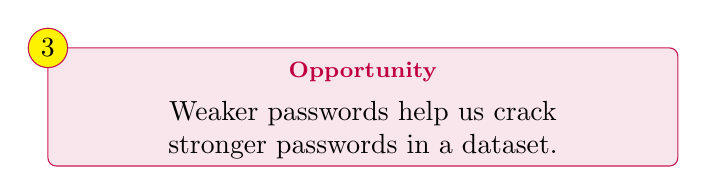
\begin{tikzpicture}
    \def\gridwidth{8}
    \def\gridheight{1.5}

    % Draw the main grid
    \draw[fill=purple!10, draw=purple!90, rounded corners=3pt,] (0,0) rectangle (\gridwidth,\gridheight);

    \node[align=center, text=purple, font=\footnotesize] (box1) at (\gridwidth/2,\gridheight-0.3) {\bf Opportunity};
        
    \node[below, text width=7cm, align=center] at (box1.south) {Weaker passwords help us crack stronger passwords in a dataset.};
    
    \node[circle,fill=yellow,inner sep=0pt,minimum size=0.5cm, draw=purple!90] at (0,\gridheight) {3};
\end{tikzpicture}
\end{center}

To formalise the expected information gain about words in $wwww$ or $\bm{w^4}$ structures given knowledge of words used in `w`, we utilise concepts from information theory, specifically entropy and conditional entropy. This approach quantifies the uncertainty in the $\bm{w^4}$ structures and how this uncertainty is reduced with knowledge of the `w` distributions.

Maximise expected information gain from cracking a certain structure.

\subsection*{Entropy}

Entropy (\(H\)) measures the unpredictability or randomness of a system. For a set of words \(W\), the entropy is calculated as:

\[
H(W) = -\sum_{i=1}^{n} P(w_i) \log_2 P(w_i)
\]

where \(P(w_i)\) is the probability of the \(i^{th}\) word occurring in the set, and \(n\) is the number of unique words.

\subsection*{Conditional Entropy}

Conditional entropy (\(H(W|W')\)) measures the amount of uncertainty remaining about \(W\) (the words in `wwww`) given \(W'\) (the distribution of words in `w`). It's defined as:

\[
H(W|W') = -\sum_{j=1}^{m} P(w'_j) \sum_{i=1}^{n} P(w_i|w'_j) \log_2 P(w_i|w'_j)
\]

where \(P(w_i|w'_j)\) is the conditional probability of word \(w_i\) given the word \(w'_j\), \(m\) is the total number of `w` words, and \(n\) is the total number of `wwww` structures.

\subsection*{Expected Information Gain}

The expected information gain (\(IG\)) about the words in `wwww` structures given knowledge of `w` can be calculated as the difference between the initial entropy of `wwww` and the conditional entropy of `wwww` given `w`:

\[
IG(W;W') = H(W) - H(W|W')
\]

This quantifies how much knowing the distribution of single words (`w`) reduces our uncertainty about the composition of phrases (`wwww`).

\subsection*{Applying the Formalization}

1. \textbf{Calculate \(H(W)\)}: Compute the entropy of the `wwww` structures based on their distribution. This involves analyzing the dataset to determine the probability distribution of different `wwww` structures.

2. \textbf{Calculate \(H(W|W')\)}: Compute the conditional entropy of `wwww` given `w`. This requires understanding how likely each `w` word is to appear in the `wwww` structures.

3. \textbf{Compute \(IG(W;W')\)}: Calculate the expected information gain, indicating how much knowing `w` aids in predicting `wwww`.

\subsection*{Practical Considerations}

- \textbf{Probability Estimation}: Estimating \(P(w_i)\) and \(P(w_i|w'_j)\) necessitates a thorough analysis of the dataset, considering both `w` and `wwww` distributions.

- \textbf{Complexity}: The actual combinations of `w` into `wwww` and their probabilities can be complex, requiring a detailed understanding of language patterns.

- \textbf{Data Requirements}: Accurate estimation of these probabilities and the information gain requires a large and representative dataset of both `w` and `wwww`.

%%%\section{Theory of personal information}
\begin{center}
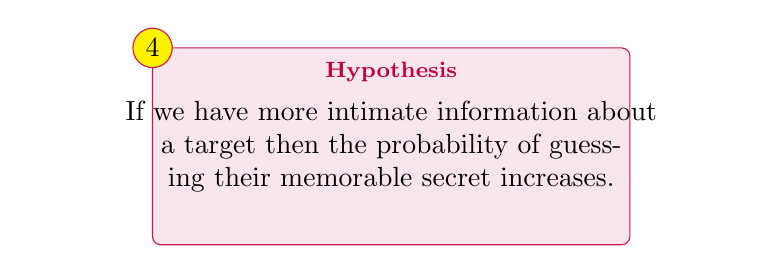
\begin{tikzpicture}
    \def\gridwidth{0.5\textwidth}
    \def\gridheight{2.5}

    % Draw the main grid
    \draw[fill=purple!10, draw=purple!90, rounded corners=3pt,] (0,0) rectangle (\gridwidth,\gridheight);

    \node[align=center, text=purple, font=\footnotesize] (box1) at (\gridwidth/2,\gridheight-0.3) {\bf Hypothesis};
        
    \node[below, text width=9cm, align=center] at (box1.south) {If we have more intimate information about a target then the probability of guessing their memorable secret increases.};
    
    \node[circle,fill=yellow,inner sep=0pt,minimum size=0.5cm, draw=purple!90] at (0,\gridheight) {4};
\end{tikzpicture}
\end{center}


It is very interesting that we embed useful information about ourselves in our chosen secrets.
\section{Mask Attack}
\label{sec::chp5::mask-attack}

Mask attack is a method of guessing a password string when you have a partial representation of it, e.g. \password{p***w0r*}, or when individual characters are brute-forced using a chosen character set. Mask attack is a crucial password cracking technique as it allows us to make assumptions about the structure of the password, and therefore reduce the search space. Such assumptions about the structures are valid and practical. Moreover, it can aid in password recovery when the user has forgotten part of the password. Mask attacks can be used with the shoulder surfing attack, especially if the attacker has only captured small segments of the password. Despite the promising nature of it, the literature on this method is sparse. \hashcat provides a rich deterministic mask attack mode, and in the academic literature, a variant of this attack is described as \textit{Conditional Password Guessing (CPG)}~\cite{pasquini_improving_2021, xu_improving_2023}. We will refer to it as \textit{Mask Attack} because of its prominent use in practice, especially since \hashcat refers to it as mask attack. The aim is to correctly guess the missing characters (denoted by ``*'').

The purpose of this section is to review existing methods and to systemise the mask attack. The methods described in~\cite{pasquini_improving_2021, xu_improving_2023} follow a similar method; however, they have three drawbacks:
\begin{enumerate}
    \item Limited comparison to \hashcat and to the point that the mask attack method in \hashcat is ignored.
    
    \item Practicality of random masking of characters.
    
    \item A flow and model of the entire guessing process is not provided and thus it avoids the most crucial aspect of password guessing--speed and candidate generation.
\end{enumerate}

The brute-force method enumerates through masked characters in order to find a correct match. This method is predominantly used in practice using \hashcat.

% We can categorise the mask attacks into: 1) Probabilistic mask attack; 2) brute-force mask attack; 3) Dictionary + mask attack.
% 
% Mask attack scenarios can be conditioned on prior knowledge about the password. Knowledge about the structure, characters, language, knowledge about the user, and etc.

\subsection{Probabilistic Mask Attack}
\begin{figure}[ht]
    \centering
    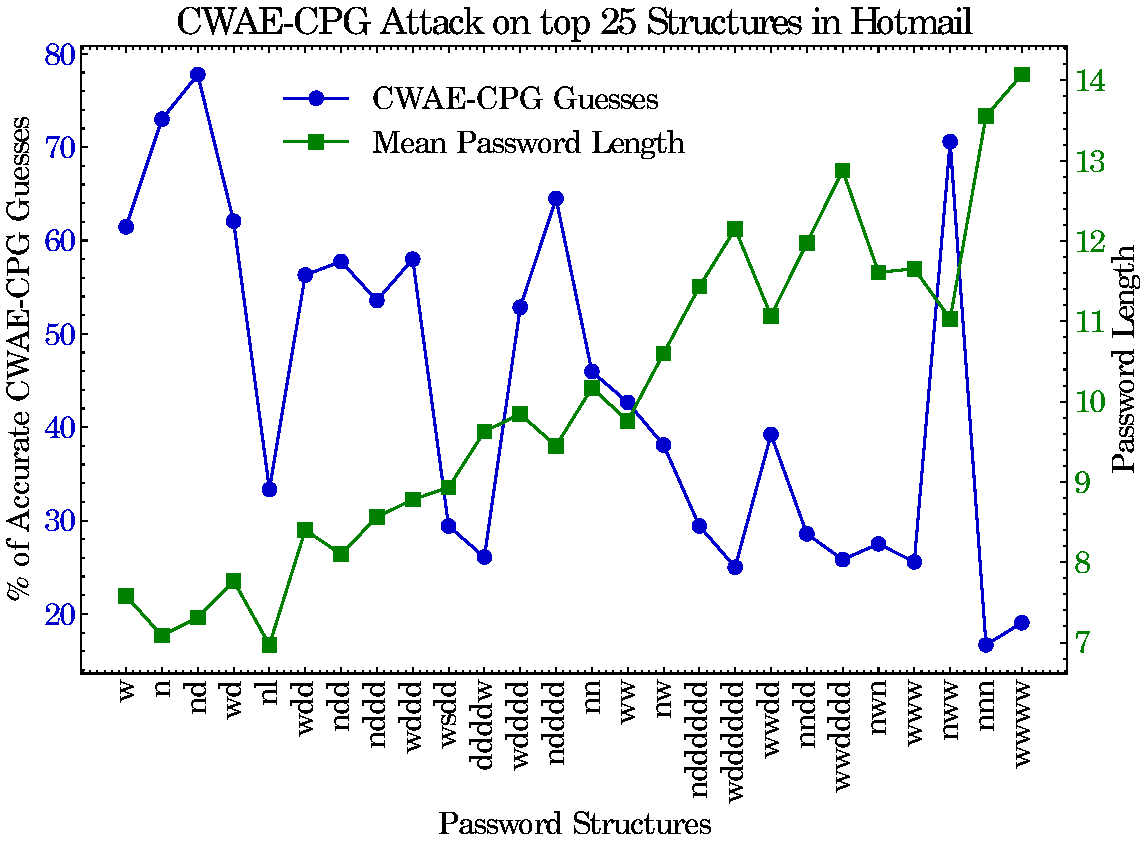
\includegraphics[scale=0.8]{figs/how_passwords/cwae_cpg_structures.pdf}
    \caption{Graph showing the percentage of guesses (left $y$-axis) with respect to the password structures in the \hmail dataset. Right $y$-axis shows the mean password length with respect to the password structures in the $x$-axis. \srcOwnFig}
    \label{fig::chp5::cwae_cpg_structures}
\end{figure}
\begin{figure}[ht]
\centering
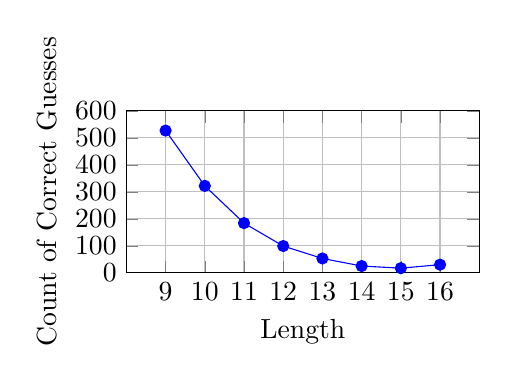
\begin{tikzpicture}
\begin{axis}[
    xlabel={Length},
    ylabel={Count of Correct Guesses},
    xmin=8, xmax=17,
    ymin=0, ymax=600,
    xtick={9,10,11,12,13,14,15,16},
    ytick={0,100,200,300,400,500,600},
    grid=major,
    width=0.5\textwidth,
    height=0.3\textwidth,
]
\addplot[color=blue, mark=*] coordinates {
    (9, 527)
    (10, 322)
    (11, 184)
    (12, 99)
    (13, 53)
    (14, 25)
    (15, 17)
    (16, 30)
};
\end{axis}
\end{tikzpicture}
\caption{Graph showing the performance of \cwaecpg against length of passwords. Using the \hmail dataset for analysis. We see a significant drop off as the length of passwords increase.}
\label{fig:mask_guess_count}
\end{figure}
\begin{table}[ht]
    \footnotesize
    \caption{Deep Learning and Probabilistic Masking Attacks literature.}
    \label{tab:my_label}
    \centering
    \begin{tabular}{ccccc}
        \toprule
        Exp & Train & Validation & Length & n \\
        \midrule
        CWAE-CPG \cite{pasquini_improving_2021} & Rockyou & Linkedin & $9 \leq L \leq 16$ & $10^7$ \\
        PassBERT \cite{xu_improving_2023} & Rockyou & NeoPets/Cit0day & $9 \leq L \leq ?$ & $10^7$ \\
        \bottomrule
    \end{tabular}
\end{table}
There are two notable models to be aware of at the time of writing: \cwaecpg uses a deep learning model based on the Wasserstein Auto-Encoder~\cite{tolstikhin_wasserstein_2019}. \passbert uses the BERT~\cite{devlin_bert_2019} architecture to model the password using the masking paradigm. These methods will often learn representation at word level, or structural patterns due to common passwords. These models condition the guess on some known characters in the password. The following shows the original password on the left and the \textit{template}\footnote{The reader may use the following website to try the masking algorithm on their own inputs: \url{https://sirvan3tr.github.io/tools/pwd/pwd_masker.html}} or masked password on the right.
\[
\text{\password{passw0rd123}} \rightarrow \text{\password{p***w0r*1*3}}
\]
The models then use deep learning techniques to learn to guess the masked characters or \textit{wild cards} (denoted by ``*''.)

We hypothesise that these methods will not do well against passphrases, or uncommon structures. For example, \password{TheTrooper} $\rightarrow$ \password{*h*****per} has too many masked characters to identify it as two words. Due to the 16 character limit as well, the model's outcome will be biased towards passphrases--which as we discussed are the strongest password structures.

We evaluated \cwaecpg\ against our labelled \hmail dataset to better understand the models performance against different password structures, the results are shown in Figure \ref{fig::chp5::cwae_cpg_structures}. For each password in the labelled \hmail dataset, we generated a template as per the \cwaecpg\ masking algorithm; then we evaluated each template (i.e. masked password) using the implementation and checkpoints released by the authors; finally for each password structure we calculated the percentage of passwords that were guessed correctly within $10^7$ guesses. Simpler structures (left side) tend to be shorter and more guessable; More complex structures (right side) tend to be longer and less guessable. Though the performance of \cwaecpgnocite\ seems correlated with the length of the password, we think the complexity is not necessarily the length but the fact that longer passwords in the dataset are composed using multiple words, dates, and names. This is further proof for NCSC's recommendation of composing these secrets using at least three random words.

Features of the training data, such as language, password structures, and date of breach, could effect the performance of the model. For example: Given a password dataset $D_t$ released at time $t$, we hypothesise that passwords containing temporal features (like years and dates) follow a time-dependent distribution $p_t(y)$ that heavily favours years closer to and preceding the release date $t$. This creates a fundamental challenge for password guessing models: when a model trained on an older dataset (e.g., $D_{2009}$) is evaluated on a newer dataset (e.g., $D_{2020}$), it encounters significant temporal distribution shift, as the training data lacks examples of passwords containing more recent years. For instance, while passwords like \password{password2018} might be common in $D_{2020}$, they would be entirely absent from $D_{2009}$, leading to poor generalization performance for passwords containing post-2009 temporal features.

%\subsection{Mask Attack Model}

\begin{figure}[t]
    \centering
    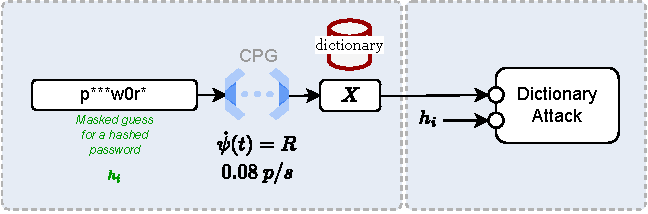
\includegraphics[scale=1.1]{figs/how_passwords/cpg.pdf}
    \caption{Data flow and model of a probabilistic mask attack or CPG. These methods thus far have randomly masked a password string and then generated a set of potential candidates. These candidates are then used to perform a dictionary attack. $\dot \psi(t)$ represents the rate of password generation. Note, an offline attack scenario is considered here.}
    \label{fig:masking-model}
\end{figure}
%The need for systematisation of mask attack is exemplified by the following. What \hashcat describes as a mask, e.g. \texttt{"?l?l?l?l?l"}, is described as a \textbf{template} in \cwaecpg and as a \textbf{pivot} in \passbert. Whilst we understand template, it is much harder to argue for the use of the term ``pivot''.
%
%A system conducting a probabilistic mask attack will use algorithms as follows.
%\begin{enumerate}[itemsep=0pt, parsep=0pt, leftmargin=12pt]
%    \item \textbf{\textsc{Mask}(1):} Let $x \in \mathcal{P}$, where $\mathcal{P}$ is the set of all possible passwords, $c_{min} \in \mathbb{N}$, and $m_{min} \in \mathbb{N}$. Define a masking function $f_1 : \mathcal{P} \times \mathbb{N} \times \mathbb{N} \rightarrow \mathcal{P}$ such that $f_1(x, c_{min}, m_{min}) = \hat{x}$, where $\hat{x}$ is the masked version of $x$, ensuring that at least $m_{min}$ characters are masked and at least $c_{min}$ characters remain unmasked.
%    
%    \item \textbf{\textsc{Mask}(2):} Given $x \in \mathcal{P}$ and $n \in \mathbb{N}$, define a masking function $f_2 : \mathcal{P} \times \mathbb{N} \rightarrow \mathcal{P}$ where $f_2(x, n) = \hat{x}$, and $\hat{x}$ is the result of masking $n$ distinct segments from the password $x$.
%    
%    \item \textbf{\textsc{Generate}(1):} Define a generation function $g_1 : \mathcal{P} \times \mathbb{N} \rightarrow 2^\mathcal{P}$, where $2^\mathcal{P}$ denotes the power set of $\mathcal{P}$, such that $g_1(\hat{x}, n) = X$, given a masked password $\hat{x}$, and $X$ is a set of $n$ potential password candidates.
%    
%    \item \textbf{\textsc{Generate}(2):} For a randomly masked password $\hat{x} \in \mathcal{P}$, define a generation function $g_2 : \mathcal{P} \rightarrow \mathcal{C}$, where $\mathcal{C}$ is the charset used to construct potential candidates, such that $g_2(\hat{x}) = y$. For example, $g_2(\text{"p***sw0rd"}) = \text{"p[l][l][l]sw0rd"}$, where $[l]$ indicates a placeholder for characters from a specified charset to be brute-forced.
%    
%    \item \textbf{\textsc{Filter}:} Define a filtering function $h : 2^\mathcal{P} \times \mathcal{P} \rightarrow 2^\mathcal{P}$, given a set of potential candidates $X \subseteq \mathcal{P}$ for masked password $x \in \mathcal{P}$, such that $h(X, x) = \hat{X}$, where $\hat{X} \subseteq X$ and $|\hat{X}| \ll |X|$. This function filters and significantly reduces the number of potential candidates by applying a set of predefined criteria or heuristics.
%\end{enumerate}

% The purpose of this section is to prove their unpracticality. The dangers of methods like this can feed into password composition policies and password complexity. The dangers are that we underestimate the real world and password guessing capabilities in the real world.

% PassBERT generates at 4.54 pwds/s, and CWAE-CPG at 0.08 pwds/s.


%   \begin{algorithm}
%     \footnotesize
%     \caption{Dynamic PCA}
%     \Comment{$\theta_{\mathrm{exp}}$ is globally given, and initially set to $\infty$.}
%     \Function{ExpandBasisIfInteresting($B$, $\Sigma$, $\vec{x}$)}{
%       \If{$\var{loss} > \theta_{\mathrm{exp}}$}{
%         $\var{loss} \assign \sqrt{\lVert \vec{x} \rVert^2 - \lVert \vec{x}^T B \rVert^2}$
%           \Comment{By Pythagoras}
%         $B, \Sigma \assign \FuncCall{Append}{$B$, $\Sigma$, $\vec{x}$}$\;
%         $B \assign \FuncCall{GramSchmidt}{$B$}$\;
%       }
%       $\theta_{\mathrm{exp}} \assign \FuncCall{UpdateLoss}{$\theta_{\mathrm{exp}}$, \var{loss}}$\;
%       \Return{$B$, $\Sigma$}\;
%     }
%     \Function{PeriodicDecompose($B$, $\Sigma$)}{
%       \If{\FuncCall{IsOneMinutePassed}{}}{
%         $B, \Sigma \assign \FuncCall{PCA}{$B$, $\Sigma$}$\;
%       }
%       \Return{$B$, $\Sigma$}\;
%     }
%     \Comment{The main function}
%     \Function{DynPCA($B$, $\Sigma$, $\vec{x}$, $s$)}{
%       $B, \Sigma \assign \FuncCall{ExpandBasisIfInteresting}{$B$, $\Sigma$, $\vec{x}$}$\;
%       $\Sigma \assign \FuncCall{UpdateCovMatrix}{$B$, $\Sigma$, $\vec{x}$, $s$}$\;
%       $B', \Sigma' \assign \FuncCall{PeriodicDecompose}{$B$, $\Sigma$}$\;
%       \Return{$B'$, $\Sigma'$}
%     }
%   \end{algorithm}

% \begin{algorithm}
% \footnotesize
% \DontPrintSemicolon
%   
%   \KwData{\\%
%   $\bm{s}$ Password string \\
%   $\bm{p}$ Probability, default=0.5 \\
%   $\bm{w}$ Minimum number of wildcards, default=5 \\
%   $\bm{c}$ Minimum number of normal characters, default=4}
%   \KwResult{A string with randomly replaced characters by wildcards '*' based on probability p, ensuring at least $w$ wildcards and $c$ characters remain unchanged.}
%   
%   \Function{CreateMask($s, p, w, c$)}{
%   %\SetKwProg{Fn}{Function}{:}{}
%   %\Fn{\FMain{password, p, w\_min, char\_min}}{
%         \If{$s.len < w + c$}{
%             \KwThrow{Password length must be at least the sum of $w$ and $c$.}
%         }
%         
%         \While{True}{
%         %\( x = \{c_1, c_2, \ldots, c_n\} \)
%         $x$ \assign s
% 
%             \For{$i = 0$ to $x.len$}{
%             $x[i] = 
%           \begin{cases} 
%            * & \text{if } \text{rand}() < p, \\
%            x[i] & \text{otherwise},
%           \end{cases}$
%             }
%             \If{$w$ $\leq$ count(* in x) $\leq s.len - c$}{
%                 \KwRet{x}
%             }
%         }
%   }
% \caption{Create a mask for the given password}
% \label{algo:probmask}
% \end{algorithm}

%Partial mask attacks, where a portion of the password is already fixed, has a significant advantage over other methods of attack. Therefore, the experiments and comparisons must reflect this.
%
%The method of masking also makes a significant difference. The methods in the literature \cite{pasquini_improving_2021, xu_improving_2023} are random masking with a probability of 0.5 as shown in Algorithm \ref{algo:probmask}. 
%
%Let us develop a practical model of an offline attack scenario given that CWAE-CPG also compared their method to other offline guessing techniques.
%
%Per our model, as seen in Figure \ref{fig:masking-model}, the secondary aim of a probabilistic masking attack is to reduce the search space from that of the deterministic masking attack (assuming we have the same mask). $|C| \ll S_d$


%%%\section{PRINCE Algorithm}
The PRINCE algorithm \cite{princeprocessor2015} (\textbf{PR}obability \textbf{IN}finite \textbf{C}hained \textbf{E}lements''), is a password guessing algorithm when given an input wordlist $W$ and a target length $n$, the algorithm generates password candidates through permuted combinations. The algorithm was introduced by Jens Steube in 2014.

Key features of the PRINCE algorithm include:

\begin{itemize}[leftmargin=11pt]
    \item Chain-based approach: PRINCE uses a chain-based method to generate password candidates. It starts with a word from a dictionary and applies various transformations (such as capitalization, leet speak, and appending numbers) to create a chain of password candidates.
    
    \item Probability-based ordering: The algorithm assigns probabilities to each transformation based on their likelihood of being used in real-world passwords. This allows PRINCE to prioritize more probable password candidates, increasing the chances of cracking the password quickly.
    
    \item Infinite length chains: PRINCE can generate password candidates of any length by recursively applying transformations to the base words, creating an infinite number of possible candidates.
    
    \item Optimized performance: The algorithm is designed to be highly optimized for modern hardware, taking advantage of GPU acceleration to perform rapid password cracking.
\end{itemize}

%%%\section{Reinforcement Learning Game}

Creating a reinforcement learning (RL) game for a password-guessing
agent involves defining the environment, states, actions, rewards, and
possibly the policy model that will learn from interactions with the
environment. Here's a mathematical formulation of such a game:

\textbf{Environment}:

\begin{itemize}
\item
  The environment \(E\) represents the set of all possible password
  hashes \(H\) and the underlying true password distribution \(P\) from
  which these hashes are generated.
\end{itemize}

\textbf{States}:

\begin{itemize}
\item
  A state \(s \in S\) encapsulates the current knowledge of the agent
  about the distribution of passwords and any partial successes in
  guessing the passwords. It could also include a history of attempts
  and their outcomes.
\end{itemize}

\textbf{Actions}:

\begin{itemize}
\item
  The action space \(A\) includes all possible password guesses that the
  agent can make. This can be partitioned into several subsets:

  \begin{itemize}
  \item
    \(A_D\) for dictionary attack actions
  \item
    \(A_M\) for masking attack actions
  \item
    \(A_G\) for actions based on passwords generated by a GAN model.
  \end{itemize}
\end{itemize}

\textbf{Rewards}:

\begin{itemize}
\item
  The reward function \(R: S \times A \rightarrow \mathbb{R}\) provides
  immediate feedback to the agent for each action. For example,
  correctly guessing a password could yield a positive reward \(r_+\),
  while incorrect guesses could yield a negative reward \(r_-\) to
  reflect the cost of time or resources.
\end{itemize}

\textbf{Policy}:

\begin{itemize}
\item
  The policy \(\pi: S \rightarrow A\) is a mapping from states to
  actions, potentially stochastic, which the agent learns in order to
  maximize its expected cumulative reward.
\end{itemize}

\textbf{Objective}:

\begin{itemize}
\item
  The goal of the RL agent is to learn a policy \(\pi^{\ast}\) that
  maximizes the expected return from any given state over a sequence of
  \(T\) time steps, often discounted by a factor \(\gamma\). The return
  \(G_t\) from a state \(s_t\) is defined as the sum of discounted
  future rewards:
\end{itemize}

\[G_t = \sum_{k=0}^{T-t} \gamma^k R(s_{t+k}, a_{t+k})\]

\textbf{Learning Problem}:

\begin{itemize}
\item
  To find the optimal policy \(\pi^{\ast}\), we seek to maximize the
  expected return from the start state \(s_0\):
\end{itemize}

\[\pi^{\ast} = \arg\max_{\pi} \mathbb{E}_{\pi}[G_0 | s_0]\]

This expectation is taken over the distribution of states visited and
actions taken under policy \(\pi\).

\textbf{Value Functions}:

\begin{itemize}
\item
  We define the state-value function \(V^\pi(s)\) as the expected return
  starting from state \(s\) and following policy \(\pi\):
\end{itemize}

\[V^\pi(s) = \mathbb{E}_\pi[G_t | s_t = s]\]

\begin{itemize}
\item
  Similarly, the action-value function \(Q^\pi(s, a)\) is the expected
  return starting from state \(s\), taking action \(a\), and thereafter
  following policy \(\pi\):
\end{itemize}

\[Q^\pi(s, a) = \mathbb{E}_\pi[G_t | s_t = s, a_t = a]\]

The agent can utilize methods such as Q-learning, policy gradients, or
actor-critic methods to learn \(V^\pi\) or \(Q^\pi\) and improve its
policy \(\pi\).

\textbf{Learning Algorithm}:

\begin{itemize}
\item
  For instance, in Q-learning, the agent would update its estimate of
  \(Q\) using the Bellman equation as:
\end{itemize}

\[Q(s_t, a_t) \leftarrow Q(s_t, a_t) + \alpha [R(s_{t+1}, a_{t+1}) + \gamma \max_{a'}Q(s_{t+1}, a') - Q(s_t, a_t)]\]

where \(\alpha\) is the learning rate.

This RL framework can then be used to simulate the process of password
guessing, allowing the agent to learn and adapt its strategy to improve
its effectiveness over time.

\subsection{The Game}

Actions:

\begin{itemize}
    \item The type of structure to choose
\end{itemize}
%%%\section{Password Similarity}
\begin{center}
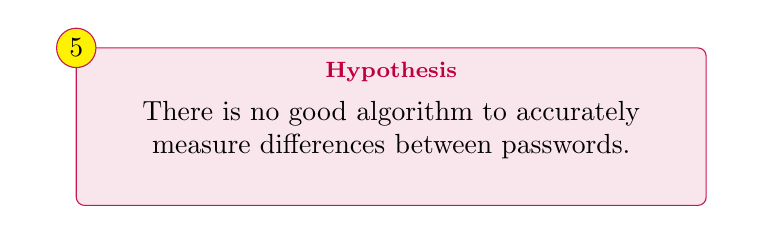
\begin{tikzpicture}
    \def\gridwidth{8}
    \def\gridheight{2}

    % Draw the main grid
    \draw[fill=purple!10, draw=purple!90, rounded corners=3pt,] (0,0) rectangle (\gridwidth,\gridheight);

    \node[align=center, text=purple, font=\footnotesize] (box1) at (\gridwidth/2,\gridheight-0.3) {\bf Hypothesis};
        
    \node[below, text width=9cm, align=center] at (box1.south) {There is no good algorithm to accurately measure differences between passwords.};
    
    \node[circle,fill=yellow,inner sep=0pt,minimum size=0.5cm, draw=purple!90] at (0,\gridheight) {5};
\end{tikzpicture}
\end{center}

The problem of password similarity is closely related to string matching. Though, measuring password similarity is more difficult than normal strings. The text transformations (such as reversals), phonetic changes, and concatenation of other words and symbols increase the difficulty.

Password similarity algorithms are important and have many use-cases. In password strength meters, we want to understand how close is the user password to existing passwords that we might deem weak. If we are developing an algorithm to generate passwords, then we might need an algorithm to measure the difference between the generated and the true password. A password similarity algorithm assumes we have a model of the password.

The classical methods such as edit distance (e.g. Levenshtein distance) are not great approximates for passwords. The transformations in passwords can greatly skew the similarity metric.

In \cite{das_tangled_2014}, Das. et al. discuss various similarity algorithms:

\begin{itemize}
    \item Distance-like. Manhattan, Cosine, etc.
    \item Edit-distance. Levenshtein, Damerau-Levenshtein functions.
    \item Token-based distance. Dice, Overlap.
    \item Alignment-like. Smith-Waterman, Neddleman Wunsch, LCS.
    \item Embedding:
        \begin{itemize}
            \item pass2path \cite{pal_beyond_2019} (Pal et al.). Uses FastText.
            \item CWAE \cite{pasquini_improving_2021} (Pasquini et al.)
            \item Other Neural Embedding (Word2Vec, GloVe, FastText, ELMo, BERT, etc.)
        \end{itemize}
\end{itemize}


\begin{itemize}
\item Distance-like
    \begin{itemize}
    \item Manhattan
    \item Cosine
    \end{itemize}
    
\item Edit-distance
\begin{itemize}
    \item Levenshtein
    \item Damerau-Levenshtein
    \item Jaro-Winkler
\end{itemize}

\item Token-based distance
\begin{itemize}
    \item Dice
    \item Overlap
\end{itemize}

\item Alignment-like
\begin{itemize}
    \item Smith-Waterman
    \item Needleman-Wunsch
    \item Longest Common Subsequence (LCS)
\end{itemize}

\item Phonetic encoding
\begin{itemize}
    \item Soundex
    \item Metaphone
\end{itemize}

\item N-gram based similarity

\item Keyboard distance metrics
\begin{itemize}
    \item Keyboard Coordinate Representation
    \item Keyboard Key Press Metric
\end{itemize}

\item Markov Chain models

\item Embedding
\begin{itemize}
    \item pass2path \cite{pal\_beyond\_2019} (Pal et al.)
    \item CWAE \cite{pasquini\_improving\_2021} (Pasquini et al.)
    \item FastText embeddings
    \item Siamese networks
\end{itemize}

\item Structural similarity
\begin{itemize}
    \item Essential Transformation Sequence (ETS)
\end{itemize}

\end{itemize}

\noindent\begin{tikzpicture}
\node[draw,rectangle,rounded corners=2pt,inner sep=10pt,outer sep=0pt] (box) {
\begin{minipage}{\columnwidth - 20pt}
\footnotesize
\centering

\textbf{Example of transformations}

\newline

\texttt{321drowssap} $\rightarrow$ \texttt{password123}

\end{minipage}
};
\end{tikzpicture}

We need to define what a similar password means. Then compare the various algorithms based on some criteria, such as complexity in time, space, accuracy, and etc.

\begin{table}[h]
\centering
\footnotesize
\caption{Time and Space Complexity of Password/String Similarity Algorithms}
\begin{tabular}{lcc}
\textbf{Algorithm} & \textbf{Time} & \textbf{Space} \\
\midrule
\multicolumn{3}{c}{\textbf{Distance-like}} \\ \hline
Manhattan & O(n) & O(1) \\
Cosine & O(n) & O(1) \\
\multicolumn{3}{c}{\textbf{Edit-distance}} \\ \hline
Levenshtein & O(mn) & O(mn) \\
Damerau-Levenshtein & O(mn) & O(mn) \\
\multicolumn{3}{c}{\textbf{Token-based distance}} \\ \hline
Dice & O(n+m) & O(n+m) \\
Overlap & O(n+m) & O(n+m) \\
\multicolumn{3}{c}{\textbf{Alignment-like}} \\ \hline
Smith-Waterman & O(mn) & O(mn) \\
Needleman-Wunsch & O(mn) & O(mn) \\
LCS & O(mn) & O(mn) \\
\multicolumn{3}{c}{\textbf{Embedding}} \\ \hline
Neural Embedding & O(n) (training) & O(n) \\
Neural Embedding & O(n) (inference) & O(n) \\
\bottomrule
\end{tabular}
\end{table}

\begin{enumerate}
\item Word2Vec (Word-level):
\begin{itemize}
\item Technique: Word2Vec uses a shallow neural network to learn word embeddings. It comes in two flavors: Continuous Bag-of-Words (CBOW) and Skip-gram. CBOW predicts a target word given its context, while Skip-gram predicts the context words given a target word.
\item Difference: Word2Vec is a straightforward and computationally efficient model that captures semantic and syntactic relationships between words.
\end{itemize}


Copy code
\item GloVe (Word-level):
\begin{itemize}
    \item Technique: GloVe (Global Vectors) learns word embeddings by factorizing a matrix of word co-occurrence statistics. It combines global matrix factorization and local context window methods.
    \item Difference: GloVe takes into account global word-word co-occurrence statistics, which can capture more global relationships compared to Word2Vec.
\end{itemize}

\item FastText (Word-level and Character-level):
\begin{itemize}
    \item Technique: FastText is an extension of Word2Vec that includes character-level information. It represents each word as a bag of character n-grams, allowing it to capture subword information and handle out-of-vocabulary words.
    \item Difference: FastText can generate embeddings for unknown words based on their character n-grams, making it useful for morphologically rich languages and handling rare or misspelled words.
\end{itemize}

\item ELMo (Character-level):
\begin{itemize}
    \item Technique: ELMo (Embeddings from Language Models) generates word embeddings using a bidirectional LSTM trained on a large text corpus. It captures context-dependent word representations by considering the entire sentence.
    \item Difference: ELMo provides dynamic word embeddings that change based on the context in which the word appears, allowing it to capture polysemy and contextual information.
\end{itemize}

\item BERT (Subword-level):
\begin{itemize}
    \item Technique: BERT (Bidirectional Encoder Representations from Transformers) uses a transformer architecture to learn contextual word representations. It is trained on a masked language modeling task and a next sentence prediction task.
    \item Difference: BERT captures bidirectional context and can generate different representations for the same word based on its surrounding context. It uses subword tokenization to handle out-of-vocabulary words.
\end{itemize}

\item GPT (Subword-level):
\begin{itemize}
    \item Technique: GPT (Generative Pre-trained Transformer) is a language model that uses a transformer decoder architecture. It is trained on a large corpus of text to predict the next word in a sequence.
    \item Difference: GPT is a unidirectional model that generates embeddings based on the previous context. It can be fine-tuned for various downstream tasks such as text generation and classification.
\end{itemize}

\item CharacterBERT (Character-level):
\begin{itemize}
    \item Technique: CharacterBERT is a variant of BERT that operates directly on character-level input. It uses a character-level CNN and a transformer encoder to learn character-level embeddings.
    \item Difference: CharacterBERT can handle out-of-vocabulary words and capture subword information without explicit tokenization. It is particularly useful for languages with complex morphology.
\end{itemize}

\item Flair (Character-level):
\begin{itemize}
    \item Technique: Flair embeddings are generated using a character-level language model trained on a large corpus. They capture contextual information and can be combined with other types of embeddings.
    \item Difference: Flair embeddings are contextual and can be used to represent words, sentences, or documents. They have shown strong performance on named entity recognition and text classification tasks.
\end{itemize}
\end{enumerate}

\begin{enumerate}
\setcounter{enumi}{8}
\item RoBERTa (Subword-level):
\begin{itemize}
\item Technique: RoBERTa (Robustly Optimized BERT Pretraining Approach) is an optimized version of BERT. It uses dynamic masking, larger batch sizes, and more training data to improve performance.
\item Difference: RoBERTa removes the next sentence prediction task and uses only the masked language modeling objective. It also trains on longer sequences and achieves better performance than BERT on various tasks.
\end{itemize}


Copy code
\item XLNet (Subword-level):
\begin{itemize}
    \item Technique: XLNet is an autoregressive language model that uses a permutation language modeling objective. It captures bidirectional context by maximizing the expected likelihood over all permutations of the factorization order.
    \item Difference: XLNet combines the advantages of autoregressive models like GPT and autoencoding models like BERT. It can handle dependencies between masked positions and achieves state-of-the-art performance on several benchmarks.
\end{itemize}

\item ALBERT (Subword-level):
\begin{itemize}
    \item Technique: ALBERT (A Lite BERT) is a lightweight variant of BERT that uses parameter-reduction techniques. It employs factorized embedding parameterization, cross-layer parameter sharing, and a sentence ordering prediction task.
    \item Difference: ALBERT significantly reduces the number of parameters compared to BERT while maintaining comparable performance. It is designed to be more memory-efficient and faster to train.
\end{itemize}

\item ELECTRA (Subword-level):
\begin{itemize}
    \item Technique: ELECTRA (Efficiently Learning an Encoder that Classifies Token Replacements Accurately) is a transformer-based model that uses a replaced token detection objective. It trains a discriminator to predict whether each token in the input is original or replaced by a generator.
    \item Difference: ELECTRA is computationally efficient and achieves strong performance on various natural language processing tasks. It is particularly effective for tasks that require fine-grained linguistic knowledge.
\end{itemize}

\item Longformer (Subword-level):
\begin{itemize}
    \item Technique: Longformer is a transformer-based model designed to handle long sequences. It uses a combination of a local self-attention mechanism and a global attention mechanism to process long documents efficiently.
    \item Difference: Longformer can handle sequences of up to 4,096 tokens, making it suitable for tasks that require processing long-range dependencies, such as document classification and question answering.
\end{itemize}

\item ConveRT (Subword-level):
\begin{itemize}
    \item Technique: ConveRT (Conversational Representations from Transformers) is a lightweight conversational reparameterization of BERT. It uses a dual-encoder architecture and a contrastive loss function to learn representations for conversational tasks.
    \item Difference: ConveRT is specifically designed for conversational AI and achieves strong performance on tasks such as response selection and intent classification while being computationally efficient.
\end{itemize}
\end{enumerate}

\subsection{Related Work}



%%%\section{Taxonomy}

\begin{figure*}[ht]
    \centering
    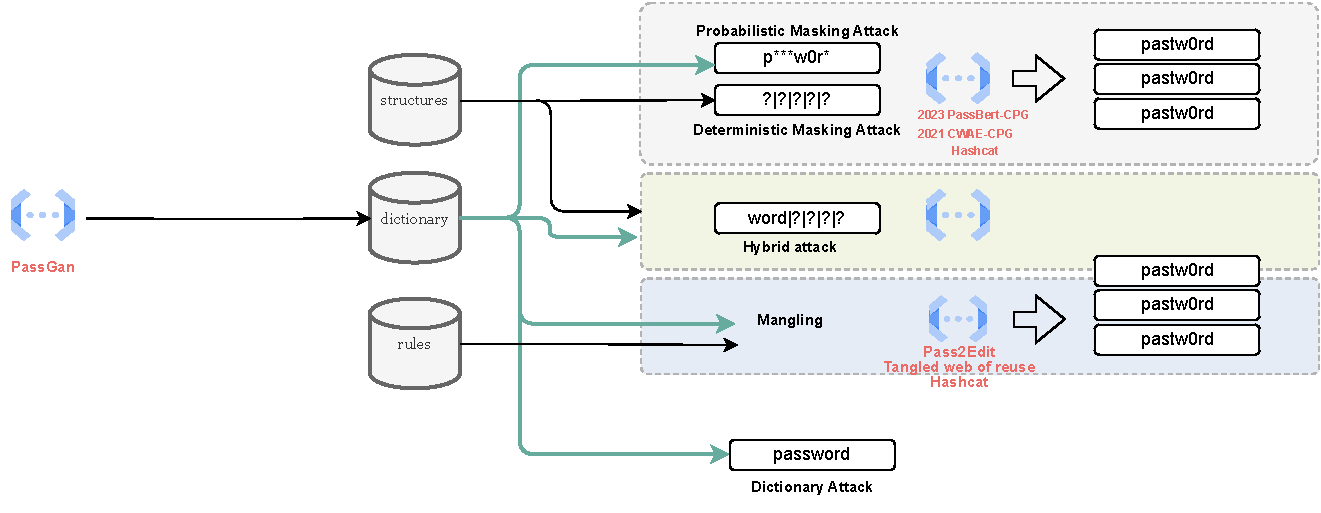
\includegraphics[scale=0.7]{figs/how_passwords/mindmap_structure2.pdf}
    \caption{Caption}
    \label{fig:enter-label}
\end{figure*}

We can compare the prior literature on password guessing using two methods: 1) comparison using implementation methodology (e.g. probabilistic vs deep learning methods); 2) method and type of attack (e.g. offline vs online attack).

Most human-chosen secrets are susceptible to pre-image attack: Given some hash value, $h$, find an input $m$ such that $\textbf{H}(m) = h$, where $\textbf{H}$ is some hash function. Consider $m$ to be the password or the memorised secret, then the argument is that it is computationally feasible to guess $m$. So, memorable secrets are not pre-image resistant. This chapter analyses the methods used to calculate the pre-image. The methods of attacks mentioned here are those that specifically target the weakness of the password--their guessability. So, it is usually the attacker v.s. a hash in two scenarios: 1) the attacker has the hash and is not limited to the number of guesses it can make; 2) the attacker does not have the hash (online attack) and is rate limited to the number of guesses. We can add two more scenarios: 1) the attacker knows the victim or has useful information about them; 2) the other attacker does not know the victim (e.g. trawlling attack). Figure \ref{fig:attack-types} demonstrates these scenarios visually in a matrix.

\begin{figure}[h]
    \centering
    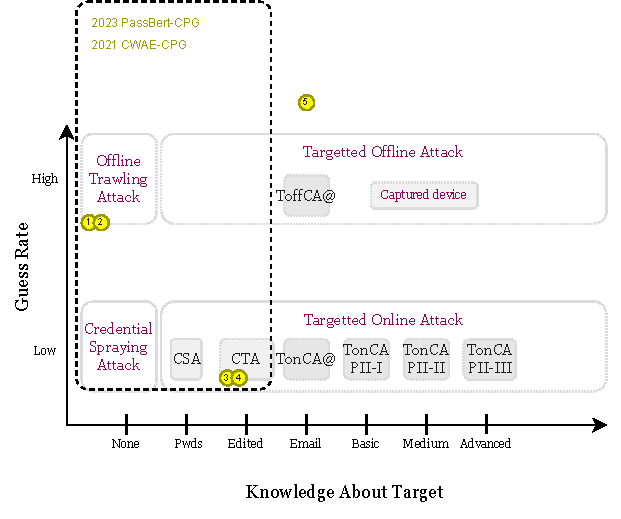
\includegraphics[scale=0.8]{figs/how_passwords/mindmap_structure.pdf}
    \caption{Caption}
    \label{fig:enter-label}
\end{figure}

\begin{figure}[h]
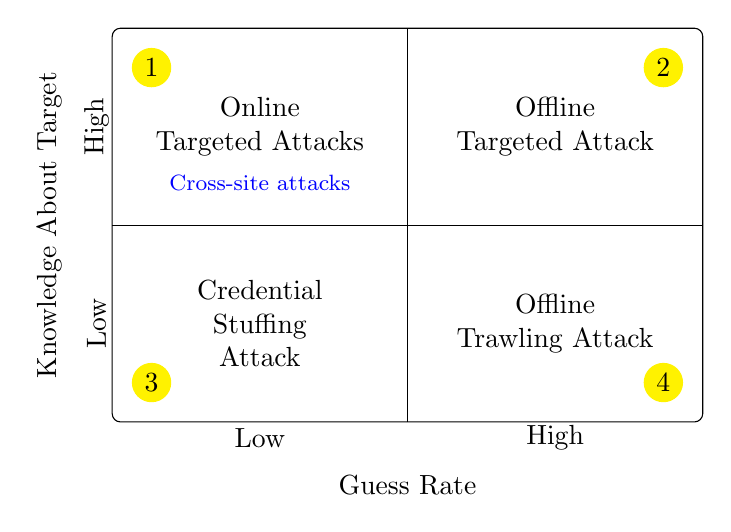
\begin{tikzpicture}
    % Variables for the grid size
    \def\gridwidth{7.5}
    \def\gridheight{5}

    % Draw the main grid
    \draw[rounded corners=3pt] (0,0) rectangle (\gridwidth,\gridheight);
    
    % Draw the dividing lines
    \draw (\gridwidth/2,0) -- (\gridwidth/2,\gridheight);
    \draw (0,\gridheight/2) -- (\gridwidth,\gridheight/2);
    
    % Labels for the attack types
    \node[align=center] (box1) at (\gridwidth/4,3*\gridheight/4) {Online\\Targeted Attacks};
    \node[align=center] at (3*\gridwidth/4,3*\gridheight/4) {Offline\\Targeted Attack};
    \node[align=center] at (\gridwidth/4,\gridheight/4) {Credential\\Stuffing\\Attack};
    \node[align=center] at (3*\gridwidth/4,\gridheight/4) {Offline\\Trawling Attack};

    \node[below, text=blue, font=\footnotesize] at (box1.south) {Cross-site attacks};
    
    % Labels for the axes
    \node[align=center] at (\gridwidth/2,-0.8) {Guess Rate};
    \node[align=center, rotate=90] at (-0.8,\gridheight/2) {Knowledge About Target};
    
    % Axis numbers
    \node[align=center] at (\gridwidth/4,-0.2) {Low};
    \node[align=center] at (3*\gridwidth/4,-0.2) {High};
    \node[align=center, rotate=90] at (-0.2,3*\gridheight/4) {High};
    \node[align=center, rotate=90] at (-0.2,\gridheight/4) {Low};


    % Circles with numbers
    % Upper left
    \node[circle,fill=yellow,inner sep=0pt,minimum size=0.5cm] at (0.5,\gridheight-0.5) {1};
    % Upper right
    \node[circle,fill=yellow,inner sep=0pt,minimum size=0.5cm] at (\gridwidth-0.5,\gridheight-0.5) {2};
    % Lower left
    \node[circle,fill=yellow,inner sep=0pt,minimum size=0.5cm] at (0.5,0.5) {3};
    % Lower right
    \node[circle,fill=yellow,inner sep=0pt,minimum size=0.5cm] at (\gridwidth-0.5,0.5) {4};

\end{tikzpicture}
\caption{Categories of attacks based on the attack rate (available to the attacker) on the horizontal axis and the amount of knowledge the attacker has about the target on the vertical axis. High attack rate signifies that the attacker has access to the target's hash. A low attack rate means that the attacker is trying to attack a hash through a website service that is rate limited.}
\label{fig:attack-types}
\end{figure}

\subsection{Models}

A guessing attack can either be completely generative or an edit function. Masking (normal and hybrid) and mangling attacks are can be described as edit functions, as they are taking a password or a structure and editing it.

\paragraph

\subsection{Context of Attack}
\paragraph*{Offline attacks}


\paragraph*{Cross-site attacks}
\begin{enumerate}
\item
  \textbf{Cross-site password attack.} Given two datasets with the same
  set of unique users but different passwords, e.g.Rockyou and
  000webhost, how many of the 000webhost passwords can I guess if I use
  the respective user's password from the Rockyou dataset?
  \item \textbf{Basic cross-site PII attack}. This attack is similar to the
    cross-site password attack but now we use more information to guess
    the password. Basic information such as name, date of birth, email,
    and other information that might be typically in a breached dataset.
  \item \textbf{Advanced cross-site PII attack}. This attack will utilise
    other information about the user in order to guess the password. For
    example information gathered from social media platforms.
\end{enumerate}

%\begin{Shaded}
%\begin{Highlighting}[]
%\NormalTok{rockyou\_data }\OperatorTok{=}\NormalTok{ \{}\StringTok{\textquotesingle{}bob@gmail.com\textquotesingle{}}\NormalTok{: }\StringTok{\textquotesingle{}password0!\textquotesingle{}}\NormalTok{, ...\}}
%\NormalTok{webhost\_data }\OperatorTok{=}\NormalTok{ \{}\StringTok{\textquotesingle{}bob@gmail.com\textquotesingle{}}\NormalTok{: }\StringTok{\textquotesingle{}p4ssword!0\textquotesingle{}}\NormalTok{, ...\}}
%
%\NormalTok{right\_guesses }\OperatorTok{=} \DecValTok{0}
%\ControlFlowTok{for}\NormalTok{ email, password }\KeywordTok{in}\NormalTok{ rockyou\_data:}
%\NormalTok{    guessed }\OperatorTok{=}\NormalTok{ guess\_password(prev\_pwd: password, iterations: }\DecValTok{100}\NormalTok{)}
%    \ControlFlowTok{if}\NormalTok{ guessed:}
%\NormalTok{        right\_guesses }\OperatorTok{+=} \DecValTok{1}
%        
%\NormalTok{percentage\_guessed\_right }\OperatorTok{=}\NormalTok{ (right\_guesses }\OperatorTok{/} \BuiltInTok{len}\NormalTok{(webhost\_data)) }\OperatorTok{*} \DecValTok{100}
%\end{Highlighting}
%\end{Shaded}


\hypertarget{evaluation-criteria}{%
\subsection{Evaluation criteria}\label{evaluation-criteria}}

\begin{itemize}
\item
  Guessing performance
\item
  Running time
\item
  Generation capacity
\item
  Duplicate rate
\item
  Model Size
\item
  Training time
\end{itemize}

\hypertarget{future-work}{%
\subsection{Future work}\label{future-work}}

\begin{itemize}
\item
  Real world attackers seldom use the techniques offered by Academia.
  The Hashat write up 2023, used a PCFG method. The work in
  {[}@pasquiniReducingBiasModeling2021{]} (Pasquini et al.~2021) argue
  that real world attackers use more pragmatic methods such as
  dictionary-based attacks. Their argument is that domani-knowledge is
  requried. So they develop new dictionary-based attacks:
  \textbf{adaptive mangling ruels attack} and \textbf{dynamic guessing
  strategies}.

  \begin{itemize}
  \item
    ``dictionary attacks describe password distributions by factorizing
    guesses into two main components---a dictionary word w and a
    transformation rule r. Here, the word w acts as a semantic base,
    whereas r is a syn- tactic transformation that aims at providing a
    suitable guess through the manipulation of w.''
  \item
    Dynamic dictionary attack

    \begin{itemize}
    \item
      THe authors argue that distribution of passwords could differ
      because of language, community interests and imposed policies.
    \item
      dynamic attacker is an adversary who changes his guessing strategy
      according to the attack's success rate
    \item
      we dynamically augment the dictionary during the attack using the
      guessed passwords.
    \end{itemize}
  \item
    The paper doesn't go into the details of the hits that worked and
    what could be done to improve it more.
  \end{itemize}
\end{itemize}


\hypertarget{offline-attack}{%
\subsection{Offline Attack}\label{offline-attack}}

\begin{table*}
\caption{Trawling attacks}
\begin{tabularx}{\textwidth}{clp{3cm}p{3cm}cc}
\toprule
Year & Model & Data & Comparison & Method & Code \\
\midrule
2023 & RFGuess & Rockyou
000webhost & FLA
PCFG
Markov & Random Forest Trees & Link \\
2023 & PassBERT-CPG & Rockyou
000webhost
Neopets
Cit0day
Rockyou-2021 & Hashcat (rule-based)
ADaMs
Vanilla BERT & Transformer & N/A \\
2022 & G-pass & & & GAN & N/A \\
2022 & STAT22 & & Markov
PCFG
Hashcat
JtR & & N/A \\
2022 & OMECDN & & OMEN
PassGAN & Markov & N/A \\
2022 & GNPassGAN & Rockyou
phpbb & PassGAN & GAN & Link \\
2021 & CPG21 & & PassGAN & GAN & Link \\
2021 & AdaMs & 4iQ & Hashcat & ANN & Link \\
2019 & PassGAN & Rockyou
LinkedIn & Markov
Hashcat
PCFG
FLA
JtR & GAN & Link \\
2016 & FLA & & PCFG
Markov
JtR
Hashcat & RNN & Link \\
2009 & PCFG & & & & Link \\
2005 & Markov & & & & \\
N/A & Hashcat & N/A & N/A & N/A & N/A \\
\bottomrule
\end{tabularx}
\end{table*}

Offline attack assumes that we are not limited to the number of guesses
we can make and therefore we have the password hash to attack. For
example, a leaked database belonging to eHarmony site has 1.5million md5
hashes but no cleartext. A clear tool in this category is Hashcat.

Dictionary attack uses a large list of generated passwords to guess and
crack a hashed password. Trawling attack is a type of password-guessing
attack where a large combination of words are used to match the target
password with. In the literature the aim of trawling attack is to create
a wordlist. In this section we will do a review of the

\textbf{Markov n-gram} \cite{narayanan_fast_2005}

\textbf{Probabilistic context-free grammar (PCFG)} \cite{weir_password_2009}

\textbf{RFGuess} \cite{wang_password_2023} (2023) uses Random Forest
trees to generate passwords. The authors have falsely called this trawlling attack, the two algorithms sit between \textit{Credential Stuffing Attack} and \textit{Online Targeted Attack}. The authors claim that is similar to the
Markov 7-gram model without much comparison to the Markov 7-gram models
in the results section. They compare the model to PCFG, Markov and FLA.
Experiment scenarios are split between different sites (cross-sites) and
inter-site, where they use a portion of the leaked password set to the
training and the remaining portion for testing. RFGuess uses the Rockyou
and 000webhost dataset for the trawling attack. The results are
inconclusive in our opinion. With a lack of tabular data it is difficult
to judge the differences in the models. The different graphs show
RFGuess performing similar to worse than its counterparts. The claim
that \emph{`RFGuess outperforms all its counterparst in intra-site
guessing scenarios'} can not be seen in the results. Lastly, the authors
falsely claim that RFGuess is suitable for online password guessing
scenarios. The results (in Fig 6 and 7 in their paper) invalidates this
statement. Their claim that online guessing is unavoidable and its
success is rather high is also false. Majority of websites implement
rate limiting in their authentication systems. In summary, the use of
Random Forest Trees for trawling attack is inconclusive from this paper
and the results are deemed to be worse than their counterparts.

\textbf{PassBERT} \cite{xu_improving_2023} introduces
three distinct attack methodologies: Conditional Password Guessing
(CPG), Targeted Password Guessing (TPG), and Adaptive Rule-based
Password Guessing (ARPG). This study focuses primarily on the
non-targeted trawling attack, namely CPG. The data pre-processing phase
involves the exclusion of hashed passwords, the elimination of non-ASCII
character passwords, and the removal of passwords exceeding 32
characters in length. Passwords undergo tokenization at the character
level, incorporating the {[}CLS{]} and {[}SEP{]} tokens to signify the
commencement and termination of sequences, respectively. The model's
pre-training employs the Rockyou-2021 dataset, utilizing a random
sampling of 60 million entries. On average, PassBERT demonstrates a
password generation rate of 4.54 passwords per second. A comparative
analysis is conducted with the Context Wasserstein Autoencoder (CWAE) as
documented in Pasquini et al.~(2021)  \cite{pasquini_improving_2021}. Notably, the referencing
of this model appears to be erroneous. The rationale provided by the
authors for selecting CWAE over Pass2path (Pal et al., 2019) \cite{pal_beyond_2019} and ADaMs (Pasquini et al.,
2021) \cite{pasquini_reducing_2021} is predicated on CWAE's
superior performance. The reproducibility of password guessing attacks
presents significant challenges. Efforts to contact the original authors
for access to the model and its weights proved futile, further
complicating the replication process.

\textbf{CWAE} \cite{pasquini_improving_2021} This paper
proposes using representation learning with deep generative models like
GANs and autoencoders for password guessing. The authors train these
models on leaked password datasets like RockYou to learn a latent
representation of passwords that captures semantic relationships. They
introduce two novel password guessing frameworks - Conditional Password
Guessing (CPG) which can generate biased guesses, and Dynamic Password
Guessing (DPG) which adapts the guessing strategy based on successfully
guessed passwords. CPG allows generating passwords matching arbitrary
templates or biases using the strong locality property of the latent
space. DPG leverages the weak locality to reduce the covariate shift
between train and test password distributions. The authors compare these
techniques against probabilistic guessers like OMEN, PCFG and FLA on
biased test sets created from LinkedIn data. They show CPG can
efficiently generate rare biased guesses unlike other methods. DPG
adapts and outperforms static attacks on diverse leaks like Youku and
Zomato exhibiting distribution shifts.

\begin{itemize}
\item
  \textbf{Trawling guessing} means that the attacker does not care who
  the specific target is.
\item
  Uses 13 large password datasets. 241.27 million pwds.
\item
  Compares it with PCFG, Markov, and FLA.
\item
  There are no tabular review of the data! hard to compare the models.
\item
  The improvement on other models is negligible.
\item
  Are they lacing the data with the test data? \emph{``Since the
  attacker is smart and will constantly improve her training set to make
  it as close as possible to the test set (to improve her
  success-rates), our intra-site experimental methodology just reflects
  this sit- uation''}
\end{itemize}

\hypertarget{methods}{%
\subsection{Methods}\label{methods}}

\begin{itemize}
\item
  \textbf{GAN}

  \begin{itemize}
  \item
    \textbf{\passgan}

    \begin{itemize}
    \item
      They referenced but did not compare the results with FLA?
      \href{https://github.com/brannondorsey/PassGAN}{According to this
      repo}. It is likely to underperform both the RNN and Markov-based
      approaches.
    \end{itemize}
  \item
    \textbf{CPG} (Conditional password guessing) and \textbf{DPG}
    (dynamic password guessing)
    {[}@pasquiniImprovingPasswordGuessing2021{]} are GAN models and an
    improvement on \emph{PassGAN} (preprinted in 2019 but published in
    2021?).
  \item
    \textbf{REDPACK} \cite{nam_generating_2020} 
  \item
    \textbf{AdaMs} \cite{pasquini_reducing_2021}
  \item
    \textbf{GNPassGAN} \cite{yu_gnpassgan_2022}
    \begin{itemize}
    \item
      \textbf{Comparison}: Only compares to \passgan
    \item
      \textbf{Training data}: Rockyou
    \item
      \textbf{Test data}: \phpbb and a disjoint subset of Rockyou.
    \item
      Experiments on two lengths

      \begin{itemize}
      \item
        Char10 \(p \leq 10\)
      \item
        Char812 \(8 \geq p \leq 12\)
        \[Matching Accuracy = \frac{\text{Count}( \text{set}(F G) \cap \text{set}(F T ))}{\text{Count}(\text{set}(F T ))}\]
      \end{itemize}
    \end{itemize}
  \end{itemize}
\end{itemize}

I have few criticisms of GNPassGAN \cite{yu_gnpassgan_2022}. It essentially uses Rockyou
dataset to generate another larger dictionary file. So, it creates a
dictionary file. But the size of the dictionary matters, the larger it
is the more hashes we have to create and therefore more time wasted on
cracking. \textbf{The order of the dictionary file} should matter.

\begin{itemize}
\item
  \textbf{Question}: Could we tailore the generated dictionary file to
  the site we are attacking? So that we have a smaller and focussed
  dictionary.
\end{itemize}

The generated (\(FG\)) file is then used to compare to \emph{phpbb's}
password list. But, what the baseline here? What if we do a straight
comparison between the two generated lists?

--- \textbf{Question}: What is the baseline? i.e.~phpbb divided by
rockyou file.

The dataset used is also very limited and small.

\begin{itemize}
\item
  \textbf{Question}: how does the generated model compare to other
  leaked datasets?
\end{itemize}

The time it takes to reach an equal password in the dataset is also
important, as mentioend before.

\begin{itemize}
\item
  \textbf{Question}: What is the ratio of generated passwords to
  duplicates per iteration?
\end{itemize}

The comparison tables are very selective, they have not shown the
comparison on the phbb dataset, only on the rockyou test. Which is
dumb\ldots{} you are taking part of the distribution away.

\begin{itemize}
\item
  \textbf{Question}: Can we guess the password for a website if we
  provide some description of the site? i.e.~not at individual level but
  at site level.
\end{itemize}

\hypertarget{targeted-guessing-attack}{%
\subsection{Targeted Guessing Attack}\label{targeted-guessing-attack}}
\cite{salimbeni_your_2023} Uses email.

%%%\section{Diffusion Framework for Password Completion}

\subsection{Theoretical Foundation}
The diffusion framework introduces a principled approach to generative modeling through a gradual noise-to-signal process. For password completion, we work in a discrete character space $\mathcal{V}^L$ where $\mathcal{V}$ is our vocabulary and L is the password length. The forward diffusion process gradually corrupts the data by replacing characters with random ones according to a schedule $\beta_t$. Formally, at each timestep t, the transition probability is:

$$q(x_t|x_{t-1}) = (1-\beta_t)\mathbb{I}(x_t = x_{t-1}) + \beta_t\text{Uniform}(\mathcal{V})$$

This creates a Markov chain $x_0 \rightarrow x_1 \rightarrow ... \rightarrow x_T$ where $x_0$ is our original password and $x_T$ is nearly random. The crucial insight is that this process is reversible, and we can train a neural network to learn the reverse transitions $p_\theta(x_{t-1}|x_t)$. For password completion, this means we can start with a partially masked password and gradually denoise it to reveal plausible completions.

\subsection{Mathematical Advantages for Password Generation}
The diffusion framework provides several key mathematical advantages for password completion. First, unlike traditional autoregressive models that generate passwords left-to-right, diffusion models can complete multiple masked positions simultaneously while maintaining consistency. The reverse process probability can be expressed as:

$$p_\theta(x_{t-1}|x_t) = \frac{p_\theta(x_t|x_{t-1})p(x_{t-1})}{p(x_t)}$$

where $p_\theta$ is parameterized by our CNN-LSTM network. This formulation allows us to sample from the posterior distribution of possible completions, leading to more diverse and realistic passwords. The loss function for training becomes:

$$\mathcal{L} = \mathbb{E}_{t,x_0,\epsilon}[\|\epsilon - \epsilon_\theta(x_t, t)\|^2]$$

where $\epsilon_\theta$ predicts the noise component at each timestep. This objective naturally handles the uncertainty in password completion by learning the entire distribution of possible completions rather than just the most likely one.

\subsection{Relationship to Password Structure}
The diffusion framework is particularly well-suited for password modeling due to the inherent structure of passwords. Let $p(x)$ be the true distribution of passwords. We can decompose this into a product of conditional probabilities:

$$p(x) = \prod_{i=1}^L p(x_i|x_{<i}, x_{>i})$$

The diffusion process allows us to learn these complex dependencies through the gradual denoising process. At each timestep t, the model learns:

$$p_\theta(x_{t-1}|x_t) \approx \prod_{i \in \mathcal{M}} p(x_i|x_{\neg i}, t)$$

where $\mathcal{M}$ is the set of masked positions and $x_{\neg i}$ represents all positions except i. This formulation is particularly powerful because:

1. It captures the dependency structure between characters in passwords through the joint distribution
2. The gradual denoising process allows the model to learn both local and global password patterns
3. The stochastic nature of the process enables sampling diverse completions that respect password conventions

\subsection{Mathematical Advantages Over Alternative Approaches}
Unlike autoregressive models which factorize the probability as $$p(x) = \prod_{i=1}^L p(x_i|x_{<i})$$, or masked language models which predict all masked tokens independently, the diffusion framework offers several advantages:

$$p_\text{diffusion}(x_\text{masked}|x_\text{observed}) = \int_{x_T} \prod_{t=1}^T p_\theta(x_{t-1}|x_t)dx_T$$

This formulation allows for:
1. Iterative refinement through the denoising steps
2. Joint prediction of masked positions while maintaining consistency
3. Natural handling of uncertainty through the stochastic process
4. Better capture of complex character dependencies through the gradual denoising

The variational lower bound of the log-likelihood can be written as:

$$\log p_\theta(x_0) \geq \mathbb{E}_{q(x_{1:T}|x_0)}\left[\log \frac{p_\theta(x_{0:T})}{q(x_{1:T}|x_0)}\right]$$

This objective ensures that the model learns a rich distribution over possible completions, making it ideal for generating multiple plausible password candidates.

\section{Model Architecture and Mathematical Justification}

\subsection{Overview}
The proposed architecture combines Convolutional Neural Networks (CNNs) and Long Short-Term Memory (LSTM) networks within a diffusion framework for password completion. This hybrid approach leverages both local character patterns and long-range dependencies in password structures.

\subsection{Architecture Components}

\subsubsection{Embedding Layer}
The input password characters $$x \in \mathbb{Z}^{L}$$ (where L is the password length) are first embedded into a continuous space:

$$E(x) = W_e x + P$$

where $W_e \in \mathbb{R}^{d \times |V|}$ is the embedding matrix (|V| being vocabulary size), and P is the learned positional encoding.

\subsubsection{Time Embedding}
The diffusion timestep t is embedded using:

$$\tau(t) = W_2\sigma(W_1t)$$

where $W_1 \in \mathbb{R}^{d \times 1}$, $W_2 \in \mathbb{R}^{d \times d}$, and $\sigma$ is the SiLU activation function. This enables the model to condition on the noise level during denoising.

\subsubsection{Convolutional Layers}
The CNN component consists of L layers of 1D convolutions:

$$h_l = \text{Conv1D}(h_{l-1}) + h_{l-1}$$

with each convolution operation defined as:

$$\text{Conv1D}(h) = W * h + b$$

where * denotes the convolution operator with kernel size k=3. This captures local character patterns and n-gram-like features within passwords.

\subsection{Mathematical Justification}

\subsubsection{Local Pattern Recognition}
Passwords often contain common local patterns (e.g., "123", "pwd", "admin"). The CNN layers with kernel size 3 create a receptive field that grows with depth:

$$\text{Receptive Field Size} = 1 + 2\sum_{i=1}^{L} (k_i - 1)$$

This allows the model to capture increasingly larger n-gram patterns, which is crucial for password structure learning.

\subsubsection{Sequential Dependencies}
The bidirectional LSTM processes the sequence in both directions:

$$\vec{h_t} = \text{LSTM}_f(x_t, \vec{h_{t-1}})$$
$$\overleftarrow{h_t} = \text{LSTM}_b(x_t, \overleftarrow{h_{t+1}})$$
$$h_t = [\vec{h_t}; \overleftarrow{h_t}]$$

This captures long-range dependencies and ensures that each position has access to both left and right context, which is essential for password completion.

\subsubsection{Diffusion Process}
The diffusion process operates in the discrete character space with transition probability:

$$q(x_t|x_{t-1}) = (1-\beta_t)I + \beta_t U$$

where $\beta_t$ is the noise schedule, I is the identity matrix, and U is the uniform distribution over the vocabulary. This allows for controlled noise injection during training and structured denoising during inference.

\subsection{Advantages for Password Completion}

\subsubsection{Pattern Recognition}
The CNN layers excel at identifying common password patterns:
\begin{itemize}
    \item Character substitutions (e.g., "a" → "@")
    \item Common numerical suffixes
    \item Repeated character sequences
\end{itemize}

\subsubsection{Context Understanding}
The bidirectional LSTM enables:
\begin{itemize}
    \item Long-range character dependencies
    \item Understanding of password structure
    \item Context-aware completion
\end{itemize}

\subsubsection{Probabilistic Sampling}
The diffusion framework provides:
\begin{itemize}
    \item Controlled noise injection during training
    \item Temperature-based sampling diversity
    \item Multiple plausible completions for masked positions
\end{itemize}

\subsection{Mathematical Properties}

The architecture guarantees several important properties:

\begin{enumerate}
    \item \textbf{Permutation Invariance}: The CNN layers are position-aware through positional encodings, ensuring the model can learn position-dependent patterns.
    
    \item \textbf{Information Flow}: The bidirectional nature of the LSTM ensures that for any position i:
    $$\frac{\partial h_i}{\partial x_j} \neq 0 \quad \forall j \in [1,L]$$
    allowing gradients to flow between any pair of positions.
    
    \item \textbf{Capacity Scaling}: The model's capacity scales with password length L:
    $$\text{Parameters} \approx O(d^2 + |V|d + Ld)$$
    where d is the model dimension.
\end{enumerate}

\subsection{Time Complexity}

The computational complexity for a password of length L is:
$$O(L \cdot d^2)$$ for the CNN layers and $$O(L \cdot d^2)$$ for the LSTM, making it more efficient than the original transformer-based approach which has complexity $$O(L^2 \cdot d)$$.

\subsection{Conclusion}
This architecture combines the strengths of CNNs (local pattern recognition), LSTMs (sequential understanding), and diffusion models (controlled generation) in a mathematically principled way. The result is a model particularly well-suited for password completion, capable of learning both local patterns and long-range dependencies while maintaining computational efficiency.

\section{Markov MCTS Mask Attack}
Given a state, select a position that is masked to do the search.



\section{Hierarchical VAE for Partially Masked Password Guessing}
\begin{figure}
    \centering
\begin{tikzpicture}[
    scale=0.8,  % Scales everything to 70% of original size
    transform shape,  % This ensures node contents are also scaled
    node distance=0.5cm,
    box/.style={
        rectangle,
        draw,
        minimum width=2cm,
        minimum height=1.5cm,
        align=center,
        rounded corners=2pt
    },
    encoder/.style={
        box,
        fill=green!10
    },
    decoder/.style={
        box,
        fill=blue!10
    },
    input/.style={
        box,
        fill=gray!10
    },
    embedding/.style={
        box,
        fill=orange!10
    },
    latent/.style={
        box,
        fill=red!10
    },
    arrow/.style={
        ->,
        thick,
        >=stealth
    }
]

% Input and Embedding
\node[input] (input) {Input Password\\$x \in \mathbb{Z}^{b \times l}$};
\node[embedding, right=of input] (embedding) {Embedding\\$E(x) \in \mathbb{R}^{b \times l \times d}$};

% Encoders
\node[encoder, above right=1cm and 1cm of embedding] (struct_enc) {Structure Encoder\\$T_1(E(x)) \rightarrow z_1$\\$z_1 \in \mathbb{R}^{b \times 256}$};
\node[encoder, right=1cm of embedding] (pattern_enc) {Pattern Encoder\\$T_2(E(x)) \rightarrow z_2$\\$z_2 \in \mathbb{R}^{b \times 128}$};
\node[encoder, below right=1cm and 1cm of embedding] (char_enc) {Character Encoder\\$T_3(E(x)) \rightarrow z_3$\\$z_3 \in \mathbb{R}^{b \times 64}$};

% Latent Space Combination
\node[latent, right=1cm of pattern_enc] (latent) {Combined Latent\\$z = [z_1;z_2;z_3]$\\$z \in \mathbb{R}^{b \times 448}$};

% Decoders
\node[decoder, above right=1cm and 1cm of latent] (struct_dec) {Structure Decoder\\$D_1(z) \rightarrow \hat{y}_1$\\$\hat{y}_1 \in \mathbb{R}^{b \times l \times v}$};
\node[decoder, right=1cm of latent] (pattern_dec) {Pattern Decoder\\$D_2(z) \rightarrow \hat{y}_2$\\$\hat{y}_2 \in \mathbb{R}^{b \times l \times v}$};
\node[decoder, below right=1cm and 1cm of latent] (char_dec) {Character Decoder\\$D_3(z) \rightarrow \hat{y}_3$\\$\hat{y}_3 \in \mathbb{R}^{b \times l \times v}$};

% Connections
\draw[arrow] (input) -- (embedding);
\draw[arrow] (embedding) -- (struct_enc);
\draw[arrow] (embedding) -- (pattern_enc);
\draw[arrow] (embedding) -- (char_enc);
\draw[arrow] (struct_enc) -- (latent);
\draw[arrow] (pattern_enc) -- (latent);
\draw[arrow] (char_enc) -- (latent);
\draw[arrow] (latent) -- (struct_dec);
\draw[arrow] (latent) -- (pattern_dec);
\draw[arrow] (latent) -- (char_dec);

% Legend
% \node[below=2cm of input, align=left] (legend) {
%     \begin{tabular}{ll}
%         $b$: batch size & $l$: sequence length\\
%         $d$: embedding dimension & $v$: vocabulary size
%     \end{tabular}
% };

% Title
% \node[above=0.5cm of input] {\Large Password Model Architecture};

\end{tikzpicture}
    \caption{Model Architecture}
    \label{fig:hvae-architecture}
\end{figure}
This section presents a novel approach to password analysis using a multi-decoder variational autoencoder (VAE) architecture. The model incorporates structural, pattern-based, and character-level understanding of passwords through a specialized hierarchical latent space representation as shown in \ref{fig:hvae-architecture}.

[to be continued...]


\section{Discussion}
\label{sec::chp5::discussion}

Going beyond surveys, systematising the knowledge of password guessing algorithms can be highly beneficial to future researchers--our reasoning is as follows.

Our continued understanding of passwords remains critical, as passwords remain the most adopted method of user authentication. The adoption of password-less authentication has remained slow, and we foresee that password will remain the leading authentication system over the next decade. Our continued understanding of it is vital for national security, too. The growth in password attacks and data breaches provides more reasoning on why we should continue research on password security.

The work in this chapter can guide future research efforts. We have identified limitations in previous approaches and various future research efforts. Insights from this analysis can inform the design and development of new authentication systems. 

Password security encompasses various issues that might be relevant to other disciplines. It touches on human-computer interaction (HCI), information security, human psychology, user experience design (UX), and cryptography. Having a common understanding can foster collaboration. This literature can also serve as a source of education.

The days of passwords are not yet over as most systems and web applications still use passwords. Passwords will continue to be used for offline systems, secure and privately networked systems, and for ad hoc usage such as password-protecting files or folders. Password-less schemes have had a slow adoption rate. The adoption of the Web Authentication API (WebAuthn) has been slow, though Passkeys have shown promise because of their usability. For these reasons, we must continue to invest in password security through further research. The purpose of this chapter is to increase the pace of password-security research.

%\subsection{Ethical Considerations}
%Our work can be argued benefits both researchers and malicious actors. However, we have shown in many instances that the techniques used in academia are rarely practical. Most practical advances in password guessing is done in private or through open-source tooling. If the work is not practical then it has no use, therefore this paper brings awareness to that fact in order to increase their comparison for real world usage.
%
%Research on password guessing increases our awareness and allows us to create better security. We can create better password strength meters (PSM) and password composition policies (PCP).

\section{Summary}
\label{sec::chp5::summary}

This chapter has provided a comprehensive systematisation of knowledge (SoK) of password guessing algorithms, bridging the gap between academic research and practical applications.

First, we address the gap between academic approaches and industry implementations. While practical tools like Hashcat focus on generation speed and hardware optimisation, academic research tends to focus on maximising successful guesses while minimising wasted attempts. We developed a novel framework for evaluating password guessing algorithms that combines both generation quality and speed. Our initial experiments revealed that sophisticated academic methods do not necessarily outperform simpler methods when both factors are considered.

We then provided a detailed overview and potential of Mask Attacks and variants of them. Although mask attacks can significantly reduce the search space and improve guessing efficiency, their effectiveness varies considerably depending on the complexity and structure of the password. The empirical evaluation demonstrated that current deep learning-based mask attack methods struggle with longer passwords and complex structures, particularly passphrases.

\noteBoxGrey{Future Work: Queueing Model}{%
  %\subsection{Queueing Model}
We model the process using a single server queue. The potential candidates are generated at near deterministic rate $\lambda$ and similarly the passwords are hashed and processed at near deterministic rate $\mu$. Therefore using Kendal's notation, the system is modelled as G/G/1. Let $\lambda(t)$ represent the arrival rate, and let $\mu(t)$ represent the hashing rate (this is typically referred to as the service rate). The utilization of our hashing server $H$ is:
\begin{equation}
    \rho = \frac{\lambda}{\mu}
\end{equation}

The utilization factor $\rho = \frac{\lambda}{\mu}$ must satisfy $\rho < 1$ for system stability, implying that the generation rate cannot exceed the processing capacity of the hashing function. 

\[
\rho = \lambda \, \mathbb{E}[S]
\]

The expected wait time in the system (queue and hashing) is given by the Kingman's approximation for our G/G/1 system.
\begin{equation}
    \mathbb{E}[W] = \frac{\rho}{1 - \rho} \cdot \frac{c_a^2 - c_s^2}{2} \cdot \mathbb{E}[S]
\end{equation}
The expected time in the system for a given password candidate:
\begin{equation}
    \mathbb{E}[T] = \mathbb{E}[S] + \mathbb{E}[W]
\end{equation}
\begin{equation}
    \mathbb{E}[T] = \left[ 1 + \frac{\rho}{1 - \rho} \cdot \frac{c_a^2 - c_s^2}{2} \right] \cdot \mathbb{E}[S]
\end{equation}
Based on, we can now calculate the expected number of password candidates in the system using Little's law:
\begin{equation}
    \mathbb{E}[N] = \lambda \mathbb{E}[T]
\end{equation}
\begin{equation}
    \mathbb{E}[N] = \rho + \frac{\rho^2(c_a^2 - c_s^2)}{2(1 - \rho)}
\end{equation}

Ideally we would like our server to be operating at maximum capacity, i.e. to maximise the resources available. This implies that our password generation should match the service rate of our server. However, we still want password candidates with high probability of inverting the hash function. So, a better measure of password guessing algorithm would be the expected time to crack--i.e. the expected time for an algorithm to invert the hash function. This takes into consideration the resources available to us and the probability distribution of an algorithm successfully guessing a password.
}

%\noteBoxGrey{Future Work: Queueing Model}{%
%  %\subsection{Queueing Model}
We model the process using a single server queue. The potential candidates are generated at near deterministic rate $\lambda$ and similarly the passwords are hashed and processed at near deterministic rate $\mu$. Therefore using Kendal's notation, the system is modelled as G/G/1. Let $\lambda(t)$ represent the arrival rate, and let $\mu(t)$ represent the hashing rate (this is typically referred to as the service rate). The utilization of our hashing server $H$ is:
\begin{equation}
    \rho = \frac{\lambda}{\mu}
\end{equation}

The utilization factor $\rho = \frac{\lambda}{\mu}$ must satisfy $\rho < 1$ for system stability, implying that the generation rate cannot exceed the processing capacity of the hashing function. 

\[
\rho = \lambda \, \mathbb{E}[S]
\]

The expected wait time in the system (queue and hashing) is given by the Kingman's approximation for our G/G/1 system.
\begin{equation}
    \mathbb{E}[W] = \frac{\rho}{1 - \rho} \cdot \frac{c_a^2 - c_s^2}{2} \cdot \mathbb{E}[S]
\end{equation}
The expected time in the system for a given password candidate:
\begin{equation}
    \mathbb{E}[T] = \mathbb{E}[S] + \mathbb{E}[W]
\end{equation}
\begin{equation}
    \mathbb{E}[T] = \left[ 1 + \frac{\rho}{1 - \rho} \cdot \frac{c_a^2 - c_s^2}{2} \right] \cdot \mathbb{E}[S]
\end{equation}
Based on, we can now calculate the expected number of password candidates in the system using Little's law:
\begin{equation}
    \mathbb{E}[N] = \lambda \mathbb{E}[T]
\end{equation}
\begin{equation}
    \mathbb{E}[N] = \rho + \frac{\rho^2(c_a^2 - c_s^2)}{2(1 - \rho)}
\end{equation}

Ideally we would like our server to be operating at maximum capacity, i.e. to maximise the resources available. This implies that our password generation should match the service rate of our server. However, we still want password candidates with high probability of inverting the hash function. So, a better measure of password guessing algorithm would be the expected time to crack--i.e. the expected time for an algorithm to invert the hash function. This takes into consideration the resources available to us and the probability distribution of an algorithm successfully guessing a password.
%}
